% !TEX encoding = UTF-8
% !TEX TS-program = pdflatex
% !TEX root = ../relazione-finale.tex

%**************************************************************
\pagebreak
\chapter{Svolgimento dello stage}
\label{cap:descrizione-stage}
%**************************************************************

\intro{Nelle sezioni di questo capitolo parlerò dell'effettivo svolgimento dello stage: organizzazione dello
stage, analisi dei requisiti, progettazione ad alto livello, documentazione prodotta, test sviluppati e
validazione dei requisiti.}\\

%**************************************************************
\section{Organizzazione dello Stage}

La pianificazione, in termini di quantità di ore di lavoro, è stata distribuita secondo la tabella ~\ref{tab:organizzazione-stage}:
Dal momento che ho già avuto modo di trattare il lato tecnologico del progetto nel corso del percorso di studi, le ore di formazione sono 40 e le ho allocate per la formazione negli argomenti meno conosciuti, ossia la parte teorica dell'architettura a microservizi, una parte pratica di applicazione dei princìpi teorici in Node.js e il ripasso della caratteristiche tecniche del \emph{framework} React.
Il secondo macroblocco di attività riguarda l'analisi, la progettazione e l'implementazione dei servizi di comunicazione con i dispositivi. A queste attività ho allocato 120 ore, in quanto è stato necessario assegnare tempo per l'attività di ricerca del protocollo di comunicazione da implementare e analizzare i requisiti che caratterizzano il prototipo. Ho incluso nelle attività di progettazione di questo blocco anche la progettazione e realizzazione dei dispositivi "virtualizzati", la presenza dei quali mi ha permesso di effettuare i primi test dei servizi di comunicazione.
Il terzo macroblocco di attività riguarda l'analisi dell'interazione che un \emph{client} può avere con i servizi di comunicazione, permettendomi di arrivare alla progettazione e realizzazione del servizio che compone le funzionalità da offrire alla \emph{dashboard} e la \emph{dashboard} stessa.
L'ultimo blocco di attività riguarda la revisione del prototipo implementato e la sua possibile pubblicazione sulla piattaforma di Heroku\footcite{heroku}.

\begin{table}[H]
	\caption{Tabella che illustra la pianificazione delle attività dello stage}
	\label{tab:organizzazione-stage}
	\begin{tabular}{|>{\centering} m{1.5cm}|>{\centering} m{1.5cm}|m{10cm}|}
		\hline
		\multicolumn{2}{|c|}{\textbf{Durata in ore}} & \textbf{Descrizione dell'attività} \\
		\hline
		\multicolumn{2}{|c|}{40} & Formazione
	 	\begin{itemize}
			\item Architettura microservizi
			\item Node.JS orientato ai microservizi
			\item React
		\end{itemize}
		\\
		\hline
		\multirow{4}{*}{120} & & Analisi, sviluppo e implementazione servizi di comunicazione con i dispositivi IoT\\
		\cline{2-2}
		& 40 & \begin{itemize}
			\item Analisi dei protocolli \emph{open source} esistenti per i diversi dispositivi IoT
			\item Stima implementazione eventuali nuovi protocolli
			\end{itemize} \\
			\cline{2-2}
			& 80 & \begin{itemize}
			\item Progettazione dei servizi di comunicazione con i dispositivi
			\item Progettazione dei test dei servizi di comunicazione
			\item Realizzazione dei test e dei servizi di comunicazione in Node.js
		\end{itemize} \\
		\hline
		\multirow{4}{*}{120} & & Analisi, sviluppo e implementazione servizio di presentazione delle informazioni agli utenti\\
		\cline{2-2}
		& 40 & \begin{itemize}
		\item Analisi interazione utente con la \textit{dashboard}
		\end{itemize} \\
		\cline{2-2}
		& 80 & \begin{itemize}
			\item Progettazione del servizio di presentazione informazioni
			\item Progettazione dei test del servizio di presentazione
			\item Realizzazione dei test e del servizio di presentazione in React, HTML5 e CSS3.
		\end{itemize} \\
		\hline
		\multicolumn{2}{|c|}{20} & {\textit{Review} dei servizi, \textit{deploy} dei servizi su Heroku.}\\
		\hline
		\multicolumn{2}{|c|}{\textbf{Totale ore}} & {\textbf{300}} \\
		\hline
\end{tabular}
\end{table}
% Le settimane sono composte da 40 ore totali di impegno sul progetto,

\clearpage
\section*{\emph{Milestone}}
In questa sezione presento le \gls{milestone} previste per il progetto su base settimanale, associando a ciascuna \emph{milestone} i prodotti che devono essere sviluppati entro la corrispondente scadenza.
\begin{itemize}
	\item Prima settimana: Completamento delle attività di autoformazione con produzione di una breve relazione riguardante la stessa;
	\item Seconda e terza settimana: Analisi dei protocolli di comunicazione esistenti, primo ciclo di progettazione e implementazione del servizio di comunicazione, mirato all'implementazione dei dispositivi \textit{virtualizzati};
	\item Quarta e quinta settimana: Revisione analisi sui protocolli, secondo ciclo di progettazione e implementazione del servizio di comunicazione, mirato all'implementazione dei dispositivi fisici (Raspberry Pi);
	\item Sesta e settima settimana: Analisi dell'interazione utente con la \emph{dashboard}, progettazione e implementazione del servizio di presentazione;
	\item Ottava settimana: Revisione dei servizi, stesura del Manuale d'Uso e deploy (opzionale) di un ambiente di simulazione della \emph{dashboard} su Heroku.
\end{itemize}

%**************************************************************
\section{Ambiente di sviluppo}

In questa sezione sono descritte le tecnologie e gli strumenti di sviluppo che ho utilizzato per lo sviluppo del progetto, includendo la motivazione per cui ho fatto la scelta.
Nella tabella ~\ref{tab:tecnologie} è presente un sommario delle tecnologie di cui approfondisco nelle sotto-sezioni seguenti. Allo stesso modo, la tabella ~\ref{tab:strumenti} include il sommario degli strumenti che ho utilizzato per lo sviluppo del prototipo.

\begin{table}[H]
\caption{Tabella con il sommario delle tecnologie utilizzate}
\label{tab:tecnologie}
\begin{tabularx}{\linewidth}{|c|X|}
\hline
\textbf{Tecnologia} & \textbf{Descrizione}\\
\hline
Node.js & Node.js è un'ambiente d'esecuzione utilizzato per l'implementazione di applicazioni server in JavaScript. \\
\hline
React & React è una libreria per il linguaggio JavaScript il cui scopo è costruire interfacce grafiche. \\
\hline
ECMAS 2017 & ECMAScript è un linguaggio di programmazione la cui implementazione standard più conosciuta è JavaScript. \\
\hline
Jest & Jest è un \emph{framework} per l'implementazione di test per codice JavaScript. \\
\hline
ESLint & ESLint è uno strumento \emph{open source} per l'analisi statica del codice JavaScript prodotto. \\
\hline
HTML5 & HTML5 è un linguaggio di \emph{markup} per la formattazione e impaginazione delle pagine \emph{web} pubblicato come W3C Recommendation dall'ottobre 2014. \\
\hline
CSS3 & CSS3 è un linguaggio di formattazione delle pagine \emph{web}. \\
\hline
Docker & Docker è una tecnologia \emph{open source} sviluppata per semplificare il rilascio di applicazioni eseguibili nel contesto dei \emph{container}. \\
\hline
\end{tabularx}
\end{table}

\begin{table}[H]
\caption{Tabella con il sommario degli strumenti di sviluppo utilizzati}
\label{tab:strumenti}
\begin{tabularx}{\linewidth}{|c|X|}
\hline
\textbf{Strumento} & \textbf{Descrizione}\\
\hline
Atom & Atom è un \emph{editor} di testo sviluppato da \gls{GitHub} altamente personalizzabile. \\
\hline
Visual Studio Code & Visual Studio Code è un \emph{editor} di testo sviluppato da \gls{Microsoft} specificatamente per i linguaggi utilizzati nel \emph{web}. \\
\hline
Jest (\gls{CLI}) & Jest (CLI) è l'interfaccia a linea di comando per l'esecuzione dei test sviluppati con il \emph{framework} Jest. \\
\hline
Docker (engine) & Il Docker Engine è la combinazione dell'implementazione della tecnologia di containerizzazione con gli strumenti di gestione del ciclo di vita dei \emph{container}. \\
\hline
Docker (compose) & Docker Compose è lo strumento attraverso cui è possibile coordinare applicazioni eseguite su \emph{container} multipli. \\
\hline
\end{tabularx}
\end{table}

\subsection{Node.js}

Node.js è un'ambiente d'esecuzione multipiattaforma \emph{open source} per JavaScript e utilizzato per l'implementazione di applicazioni server in JavaScript.
Per consentire l'esecuzione di JavaScript lato server, Node.js utilizza il motore di esecuzione JavaScript \emph{V8} sviluppato da \gls{Google} per il \emph{browser} Chrome.
Ho riassunto gli aspetti positivi della piattaforma Node.js nei seguenti punti:
\begin{itemize}
  \item Node.js utilizza il modello \emph{event-driven} per la gestione delle operazioni di \emph{input} e \emph{output} (I/O) e in questo modo semplifica la gestione asincrona delle richieste concorrenti.
  \item Node.js utilizza JavaScript, un linguaggio di programmazione dalla sintassi semplice da imparare.
  \item Node.js utilizza npm per la gestione delle librerie dell'applicazione. Npm è il più grande registro di componenti di codice riusabile\footnote{Secondo le dichiarazioni degli sviluppatori di npm \url{https://www.npmjs.com/}}.
\end{itemize}

Come tutte le tecnologie, anche Node.js ha i suoi aspetti negativi, che presento di seguito:
\begin{itemize}
  \item Node.js non sfrutta i molti \emph{core} presenti nelle CPU moderne e quindi operazioni fortemente \gls{CPU-bound} congelano l'intero ciclo di eventi fino al termine dell'esecuzione dell'operazione.
  \item Node.js favorisce l'utilizzo del Design Pattern \emph{callback}, tuttavia in funzioni complesse si potrebbe incorrere in una eccessiva complessità nella lettura del codice.
\end{itemize}

\subsection{React}

React è una libreria per il linguaggio JavaScript il cui scopo è costruire interfacce utente.
Ho riassunto gli aspetti positivi della libreria React nei seguenti punti:
\begin{itemize}
	\item React utilizza un \gls{DOM} virtuale per disegnare le interfacce, raggiungendo performance ed efficienza elevate. Grazie alla sua struttura a componenti, un aggiornamento ad uno di essi non richiede l'aggiornamento degli altri.
	\item I componenti sviluppati possono essere riutilizzati, garantendo un aumento di produttività degli sviluppatori.
	\item I dati in React seguono un flusso unidirezionale, in cui i componenti figli non possono modificare dati dei loro genitori, semplificando la manutenzione dei componenti.
\end{itemize}

Il difetto principale che attribuisco a React consiste nella sua elevata dinamicità: dal momento che gli sviluppatori di React aggiornano repentinamente le versioni rilasciate (la versione utilizzata durante lo stage è la "16.2.0"), gli sviluppatori devono mantenere aggiornati i \emph{codebase} per tutte le nuove funzionalità inserite.

\subsection{ECMAScript 2017}

ECMAScript 2017 è un linguaggio di programmazione standardizzato la cui ratifica è avvenuta nel giugno del 2017. L'implementazione dello standard più conosciuta è JavaScript.
L'edizione 2017 dello standard porta in dote le seguenti funzionalità:
\begin{itemize}
	\item Nuova sintassi per le funzioni asincrone. La \emph{keyword} \emph{async} indica che una funzione o un metodo ritornano una Promise, ossia una classe di oggetti che evidenziano l'asincronia dell'operazione da eseguire. La \emph{keyword} \emph{await} aspetta che la funzione asincrona termini la sua esecuzione, ritornando il risultato della \emph{Promise}.
	\item Supporto iniziale per l'elaborazione \emph{multithread}, attraverso tipi di oggetti immutabili e condivisibili tra \emph{thread}.
	\item Nuovi metodi per gli oggetti esistenti nel linguaggio (enumerazione dei membri di un oggetto e ulteriori funzionalità di manipolazione di stringhe).
\end{itemize}

Nella mia analisi ho riscontrato che gli aspetti positivi consistono nei seguenti punti:
\begin{itemize}
	\item La nuova sintassi per la scrittura di funzioni asincrone rende facilmente leggibile il codice sorgente in quanto ricorda l'utilizzo di normali funzioni della programmazione sequenziale.
	\item Il supporto per l'elaborazione \emph{multithread} consente a chi ha necessità e competenza di poter sfruttare le architetture a molti \emph{core} delle moderne \gls{CPU}, favorendo l'utilizzo di JavaScript anche per la programmazione di codice parallelo per le \gls{GPU}.
	\item Poche nuove funzionalità rispetto alle edizioni precedenti permettono di imparare le nuove con maggior semplicità.
\end{itemize}
mentre gli aspetti negativi:
\begin{itemize}
	\item Con la nuova sintassi per le funzioni asincrone ho spesso dimenticato la natura asincrona del codice scritto, causando l'omissione della \emph{keyword} \emph{await}.
	\item Il supporto alla nuova edizione dello standard è presente in maniera completa solamente nelle ultime versioni dei \emph{browser} e di Node.js.\footnotemark
\end{itemize}

\footnotetext{
\begin{itemize}
	\item Tabella di compatiblità dei \emph{browser}: \url{http://kangax.github.io/compat-table/es2016plus/}
	\item Tabella di compatiblità di Node.js: \url{http://node.green/\#ES2017}
\end{itemize}}

\subsection{Jest}

Jest è un \emph{framework} per l'implementazione di test per codice scritto in JavaScript sviluppato da Facebook.
Tra gli aspetti positivi, ho riscontrato che:
\begin{itemize}
	\item Jest non richiede una configurazione, utilizzando impostazioni predefinite ottimali.
	\item Jest è una piattaforma di test completa che include strumenti di validazione dei risultati e strumenti per il \gls{mocking}.
	\item Jest comprende funzionalità per i test di regressione dei componenti scritti in React.
	\item Jest per default esegue i test parallelamente, velocizzando i processi di test.
\end{itemize}
Il difetto più grave che attribuisco a Jest consiste nella sua minor flessibilità rispetto ad altre librerie di test che permettono di sostituire le librerie utilizzate per il controllo delle asserzioni e per l'implementazione dei \emph{mock}.

\subsection{ESLint}

ESLint è uno strumento che esegue analisi del codice sorgente scritto in JavaScript alla ricerca di \emph{bug} noti, di inconsistenze di stile nella scrittura del codice e mira a mantenere il codice facilmente leggibile e manutenibile.
Gli aspetti positivi di ESLint che ho riscontrato sono:
\begin{itemize}
	\item ESLint è altamente configurabile, permettendo la definizione di regole condivise più appropriate per il proprio progetto.
	\item É supportato da molti strumenti di sviluppo.
	\item Le regole di analisi sono ben documentate, con esempi sul loro utilizzo, e gli errori emessi sono facilmente comprensibili.
\end{itemize}
L'aspetto negativo principale che ho trovato in ESLint risiede nella sua ripida curva di apprendimento per l'installazione e l'utilizzo: ESLint infatti richiede una configurazione iniziale non banale per il suo utilizzo.

\subsection{HTML5 e CSS3}

HTML5 e CSS3 sono le ultime revisioni stabili rispettivamente del linguaggio HTML e del linguaggio CSS rilasciate dalla W3C.
Gli aspetti positivi di queste tecnologie che ho riscontrato sono:
\begin{itemize}
	\item HTML5 ha il vantaggio di utilizzare una sintassi semplificata e più chiara rispetto alle versioni precedenti dello standard e permette l’integrazione con diversi formati multimediali senza utilizzare \emph{plugin} esterni.
	\item HTML5 e CSS3 sono ben diffusi e tutti i \emph{browser} più recenti li supportano anche in caso di versioni non aggiornate.
	\item HTML5 e CSS3 sono ben documentati e sono disponibili nella rete numerose risorse per il loro utilizzo ottimale.
\end{itemize}
Dato l'ambito di utilizzo delle tecnologie HTML5 e CSS3 in questo progetto, nel quale non ho vincolato ad una versione minima i \emph{browser} utilizzabili dagli utenti per la visualizzazione della \emph{dashboard}, non ho riscontrato difetti che potessero essere menzionati.

\subsection{Atom}
\label{subsec:atom}

Atom è un \emph{editor} di testo sviluppato da GitHub che può essere utilizzaato come un \gls{IDE}.
Atom durante il progetto è stato utilizzato per la stesura della documentazione associata al progetto: documenti di Analisi dei Requisiti e Specifica Tecnica, documenti di presentazione delle componenti del progetto (\emph{README} visualizzabili durante l'esplorazione del progetto su GitHub) e specifica delle interfacce di comunicazione tra i servizi.
Gli aspetti positivi che ho riscontrato nel suo utilizzo sono:
\begin{itemize}
	\item Atom è estremamente espandibile e personalizzabile, permettendo di creare un ambiente di sviluppo su misura.
	\item Atom riconosce la sintassi di moltissimi linguaggi attraverso moduli installabili.
\end{itemize}
Gli aspetti negativi che ho riscontrato sono:
\begin{itemize}
	\item Atom richiede un utilizzo della CPU elevato che ne mina la stabilità generale.
	\item Atom non si interfaccia nativamente con strumenti di \emph{debug} del codice.
\end{itemize}
Il secondo difetto riscontrato è stato il motivo per cui ho introdotto un altro strumento per la scrittura del codice sorgente del progetto.

\subsection{Visual Studio Code}

Visual Studio Code è un \emph{editor} di testo sviluppato da Microsoft per la scrittura di applicazioni \emph{web}.
Ho utilizzato Visual Studio Code per scrivere il codice sorgente del prototipo, per ispezionare il codice scritto in esecuzione (\emph{debug}) e per eseguire i test statici e dinamici sul codice.
Gli aspetti positivi che ho evidenziato durante il suo utilizzo consistono in:
\begin{itemize}
	\item elevata efficienza nell'utilizzo delle risorse, risultando uno strumento affidabile;
	\item supporto nativo per gli strumenti di \emph{debug};
\end{itemize}
Non ho riscontrato evidenti aspetti negativi per questo strumento, tuttavia, paragonandolo al precedente strumento per la scrittura testuale (~\ref{subsec:atom}), mi è risultato evidente la minor quantità di sintassi supportate e la minor personalizzazione generale dell'\emph{editor}.

\subsection{Docker (Engine e Compose)}

Docker è una piattaforma tecnologica che permette di semplificare la gestione del ciclo di vita dei \emph{container}, a partire da:
\begin{itemize}
	\item istanziazione: a partire da un file (\emph{Dockerfile}) che rappresenta le risorse necessarie alla compilazione (se necessaria) e all'esecuzione di un'applicazione containerizzata, chiamato nel gergo tecnico \emph{image}, Docker Engine permette di creare più \emph{container} della stessa applicazione, ciascuno dei quali è isolato di default dagli altri \emph{container} istanziati a partire dalla stessa \emph{image};
	\item avvio: nel momento in cui l'utente istanzia un \emph{container}, esso viene creato e avviato dal Docker Engine. Mentre il \emph{container} è in esecuzione, è possibile accedere alle funzionalità che tale \emph{container} offre, sia esso un \emph{container} con un base di dati oppure contenga un'applicazione \emph{server} o \emph{web};
	\item arresto: quando l'utente decide che le funzionalità offerte dal \emph{container} non sono più richieste, può arrestare il \emph{container} attraverso il Docker Engine: la piattaforma di Docker si occupa di salvare lo stato interno del \emph{container} (simile alla funzionalità di \emph{snapshot} delle tecnologie di virtualizzazione standard) per permettere che il container riparta nello stesso stato al successivo avvio;
	\item distruzione: quando l'utente decide di voler rimuovere il \emph{container} e tutte le risorse associate dal proprio elaboratore, istruisce il Docker Engine al fine di arrestare e rilasciare le risorse allocate per il \emph{container} considerato.
\end{itemize}
Gli strumenti offerti da Docker Compose espandono le funzionalità offerte dal Docker Engine e permettono di gestire l'esecuzione di un insieme di \emph{container} che compongono un'applicazione. Le funzionalità offerte da Docker Compose ricalcano quelle del Docker Engine, applicandole a insiemi di \emph{container}.

%**************************************************************
\section{Analisi dei Requisiti}
\label{ar}

% Approfondire l'Analisi dei Requisiti prodotta. + Analisi dei protocolli
\subsection{MQTT}
\label{subsec:mqtt}
\gls{MQTT} è un protocollo di messaggistica leggero basato sul \emph{Design Pattern} \emph{Publish/Subscribe}.
É un protocollo nato per l'utilizzo con sensori a basso consumo energetico, tuttavia è utilizzabile anche in altri scenari.
% TODO: mancano le fonti
MQTT è stato progettato tra la fine degli anni '90 e l'inizio degli anni 2000 per ambienti in cui l'affidabilità della rete non era garantita.\footcite{mqtt}

MQTT mira ad assere una soluzione semplice da implementare, per permettere la maggior copertura di dispositivi possibile.
MQTT usa messaggistica pub/sub per permettere ai dispositivi di pubblicare nella rete informazioni non predefinite.
MQTT non richiede amministrazione in quanto cerca di rispondere ad eventi inaspettati in maniera semplice e con maggior buon senso possibile.
MQTT minimizza il traffico sulla rete introducendo un \gls{overhead} sui dati minimo.
MQTT si aspetta di lavorare in reti con frequenti interruzioni, utilizzando il meccanismo dell'ultimo testamento.
MQTT si accorge repentinamente di cambiamenti dello stato della sessione.
MQTT si aspetta che i \emph{client} abbiano risorse d'elaborazione limitate.
MQTT mette a disposizione livelli di affidabilità per la trasmissione di informazioni critiche.
MQTT non fa assunzioni sulla struttura né il contenuto dei dati.

Il protocollo MQTT si basa sul principio che ogni \emph{client} pubblica messaggi, i quali hanno uno o più argomenti, nel gergo tecnico \emph{topic}.
Ogni \emph{client} può registrarsi a determinati argomenti per ricevere tutti i messaggi che altri \emph{client} pubblicano per quell'argomento. Molti \emph{client} si connettono a un \gls{broker} che funziona da intermediario, ricevendo i messaggi pubblicati e inoltrandoli a tutti i \emph{client} sottoscritti ai rispettivi argomenti.
Gli argomenti in MQTT sono trattati gerarchicamente. Questo permette la creazione di argomenti e sottoargomenti, simili alla struttura ad albero di un \emph{filesystem}.
MQTT definisce 3 livelli di qualità in base a quanto \emph{broker} e \emph{client} si impegneranno a ricevere un messaggio.
I \emph{client} decidono il livello massimo di \gls{QoS} che riceveranno.

La scala della QoS definisce i livelli 0, 1 e 2 con affidabilità crescente ma minori performance:
\begin{itemize}
	\item [0]: \emph{broker} e/o \emph{client} invieranno il messaggio al massimo una volta senza richiesta di conferma. A questo livello i messaggi vengono persi se una delle parti si disconnette;
	\item [1]: \emph{broker} e/o \emph{client} invieranno il messaggio almeno una volta con la richiesta di conferma;
	\item [2]: \emph{broker} e/o \emph{client} invieranno il messaggio una sola volta effettuando una trasmissione in 4 step.
\end{itemize}

Per esempio, se un messaggio è pubblicato con QoS 2 e il \emph{client} è sottoscritto all'argomento con QoS 0, il \emph{client} riceverà quel messaggio con QoS 0 (niente richieste di conferma, ecc).
Se un altro \emph{client} è sottoscritto allo stesso argomento con QoS 2 allora riceverà il messaggio con QoS 2 (\gls{handshake} in 4 step).
Alla connessione il \emph{client} imposta un parametro logico che rappresenta una "sessione pulita" in base a come il \emph{client} ritiene affidabile la connessione (`false` indica una connessione affidabile). Se il \emph{client} si disconnette, in tutte le sottoscrizioni con QoS 1 o QoS 2 i messaggi verranno salvati e inviati alla prossima riconnessione del \emph{client}.

\subsection{Requisiti}

Lo scopo di questa sezione è di definire i requisiti emersi dall’analisi del progetto di stage.
In questa sezione descrivo i requisiti, i casi d'uso collegati e gli attori coinvolti.

I dispositivi che ho considerato comunicano con il sistema utilizzando il protocollo MQTT (~\ref{subsec:mqtt}), perché ho ritenuto questo protocollo il più adatto per il sistema.
I motivi che mi hanno spinto a scegliere MQTT sono:
\begin{itemize}
	\item è un protocollo molto diffuso, caratteristica che mi ha facilitato molto nella ricerca di documentazione che dimostri il suo utilizzo;
	\item è un protocollo \emph{data agnostic}, ossia che non pone vincoli sulla struttura dei dati scambiati nella rete;
	\item è un protocollo efficiente in quanto trasmette informazioni con un \emph{overhead} minimo;
	\item è un protocollo che permette l'aggiunta e la rimozione di dispositivi dinamicamente, richiedendo intervento manuale minimo all'utente.
\end{itemize}

Tutti i dispositivi che compongono il sistema contengono al loro interno informazioni relative a modello, revisione, produttore e anno di produzione del dispositivo.
Ho definito "centro di controllo" quell'insieme di dispositivi responsabili della coordinazione tra i vari dispositivi connessi alla rete.
Ho inoltre suddiviso i dispositivi in due tipi principali in base alle funzionalità che essi offrono:
\begin{itemize}
	\item sensori;
	\item dispositivi che ho definito "attivi".
\end{itemize}
La funzionalità principale offerta dai sensori è l'invio periodico di informazioni legate a ciò che il sensore misura.
L'invio di informazioni periodiche avviene in automatico, secondo i parametri impostati dal produttore del sensore.
Altre due funzionalità legate alle risorse \emph{hardware} del sensore sono:
\begin{itemize}
	\item memorizzazione locale: il produttore dota il sensore di una piccola memoria riscrivibile, interrogabile direttamente producendo dati in un formato stabilito dal produttore. Nei casi d'uso presi in considerazione questa funzionalità è utile in caso di perdita di connessione o malfunzionamento del centro di controllo. Nel caso in cui questa funzionalità sia presente, il sensore provvede a trasmettere i dati raccolti alla prossima riconnessione con il centro di controllo.
	\item disconnessione forzata: il centro di controllo può richiedere ai sensori di disconnettersi dalla rete per un periodo di tempo per motivi di diagnostica o di sovraccarico della rete. Questa funzionalità richiede che il sensore abbia hardware in grado di ricevere segnali e non solo trasmetterli.
\end{itemize}

Nella tabella ~\ref{tab:funz-sensori} riassumo le funzionalità considerate per i sensori, descrivendone la frequenza di utilizzo, la modalità di attivazione e se la funzionalità è presente obbligatoriamente.

\begin{table}[H]
\caption{Tabella con funzionalità considerate dai sensori}
\label{tab:funz-sensori}
\begin{tabularx}{\linewidth}{|X|c|c|c|}
\hline
\textbf{Funzionalità dei sensori} & \textbf{Frequenza} & \textbf{Attivazione} & \textbf{Obbligatorietà} \\
\hline
Invio informazioni & Periodica & Automatica & Sì \\
\hline
Memoria locale & N.D. & Automatica & No \\
\hline
Disconnessione forzata & Su richiesta & Manuale & No \\
\hline
\end{tabularx}
\end{table}

I dispositivi attivi presentano le seguenti funzionalità:
\begin{itemize}
	\item pubblicazione di una lista degli eventi gestiti dal dispositivo;
	\item generazione di risposte agli eventi esterni;
	\item invio di informazioni sullo stato energetico del dispositivo;
	\item spegnimento del dispositivo.
\end{itemize}

La lista degli eventi gestiti è pubblicata dal dispositivo e permette di conoscere le funzionalità \emph{smart} del dispositvo.
La funzionalità di risposta agli eventi gestiti è automatica e avviene a ogni evento occorso.
Le funzionalità legate alla gestione degli eventi sono direttamente implementate dai produttori dei dispositivi.
L'invio delle informazioni sullo stato energetico del dispositivo richiede che il produttore abbia dotato il dispositivo di unità di \emph{power management} e perciò potrebbe non essere disponibile per tutti i dispositivi collegati.
Nella tabella ~\ref{tab:funz-disp-attivi} riassumo le funzionalità considerate per i dispositivi attivi.

\begin{table}[H]
\caption{Tabella con funzionalità considerate dai dispositivi attivi}
\label{tab:funz-disp-attivi}
\begin{tabularx}{\linewidth}{|X|c|c|c|}
\hline
\textbf{Funzionalità dei dispositivi attivi} & \textbf{Frequenza} & \textbf{Attivazione} & \textbf{Obbligatorietà} \\
\hline
Invio informazioni & Ad ogni evento ricevuto & Automatica & Sì \\
\hline
Risposta eventi gestiti & Su richiesta & Automatica & Sì \\
\hline
Informazioni stato energetico & Su richiesta & Manuale & No \\
\hline
Spegnimento & Su richiesta & Manuale & Sì \\
\hline
\end{tabularx}
\end{table}

I dispositivi facenti parte del "centro di controllo" presentano le seguenti funzionalità:
\begin{itemize}
	\item gestione dei dispositivi collegati al sistema;
	\item ricezione, elaborazione e memorizzazione delle informazioni utili provenienti dai dispositivi (anche per fini diagnostici);
	\item pubblicazione delle informazioni raccolte per i \emph{client} che interrogano il centro di controllo.
\end{itemize}

I dati ricevuti dal centro di controllo possono essere raccolti dai dispositivi in una forma grezza e perciò è necessario che il centro di controllo li elabori, a seconda della provenienza dei dati, al fine di renderli comprensibili anche agli umani.
Le informazioni raccolte sono messe a disposizione ai \emph{client} in tempo reale.

% ### Caratteristiche degli utenti del sistema

Prevedo che gli utenti del prototipo non abbiano alcuna competenza particolare.

% ### Piattaforma di esecuzione

La piattaforma di esecuzione del prodotto è Docker, attraverso la composizione di \emph{container}.
L'utente accede alle funzionalità del prodotto attraverso una interfaccia \emph{web}, opportunamente progettata per essere reattiva (ottimizzata per \emph{mobile}).

% ## Casi d'uso

I casi d’uso sono catalogati come:

\begin{figure}[H]
  \centering
  \[ UC[numero][caso] \]
  \begin{tabular}{@{}>{$}l<{$}l@{}}
    UC & specifica che si sta parlando di un caso d’uso;\\
    numero & è assoluto e rappresenta un riferimento univoco al caso d’uso in questione;\\
    caso & individua eventuali diramazioni all’interno dello stesso caso d’uso.\\
  \end{tabular}
\end{figure}

La breve descrizione di ciascun caso d’uso presenta:
\begin{itemize}
	\item gli attori del caso d’uso;
	\item lo scopo e la descrizione del caso d’uso.
\end{itemize}

Gli attori che ho considerato in sede di analisi consistono in:
\begin{itemize}
	\item Utente: rappresenta l'utente che interagisce con la \emph{dashboard};
	\item Dispositivi: rappresentano l'insieme di apparati collegati al sistema che forniscono i dati per popolare la \emph{dashboard};
	\item Dispositivo: rappresenta uno dei dispositivi collegati al sistema;
	\item Interfaccia proprietaria del dispositivo: rappresenta l'interfaccia proprietaria progettata dal produttore di un generico dispositivo.
\end{itemize}

% ![Sommario dei casi d'uso](./images/use_cases.png)
% <p align="center"><i>Sommario dei casi d'uso</i></p>

% uc testuale
\begin{usecase}{0}{Scenario principale}
\usecaseactors{Utente, Dispositivi}
\usecasepre{L'utente ha correttamente installato il prototipo e ha aperto la \emph{dashboard} in un \emph{browser}}
\usecasedesc{La \emph{dashboard} mostra lo stato del sistema ed evidenzia i dispositivi collegati}
\usecasepost{La \emph{dashboard} consente un'altra interazione con il sistema}
\label{uc:scenario-principale}
\end{usecase}

% uc figura
\begin{figure}[!h]
    \centering
    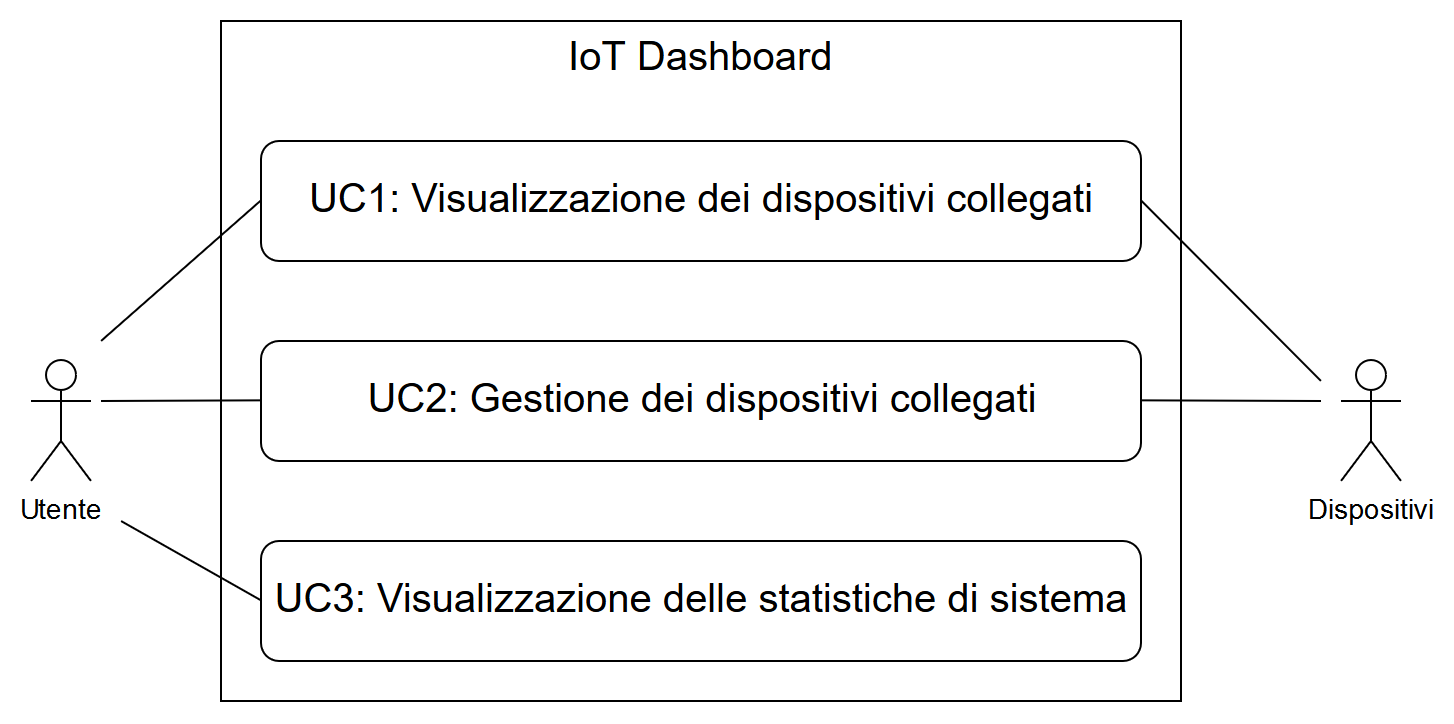
\includegraphics[width=0.9\columnwidth]{usecase/use_cases}
    \caption{Use Case - UC0: Scenario principale}
\end{figure}
% fine uc

% uc testuale
\begin{usecase}{1}{Visualizzazione dei dispositivi collegati}
\usecaseactors{Utente, Dispositivi}
\usecasepre{L'utente ha scelto di visualizzare tutti i dispositivi collegati}
\usecasedesc{L'utente interroga la \emph{dashboard} per conoscere lo stato dei dispositivi collegati}
\usecasepost{L'utente conosce lo stato di tutti i dispositivi collegati al sistema}
\label{uc:uc1}
\end{usecase}

% uc figura
\begin{figure}[!h]
    \centering
    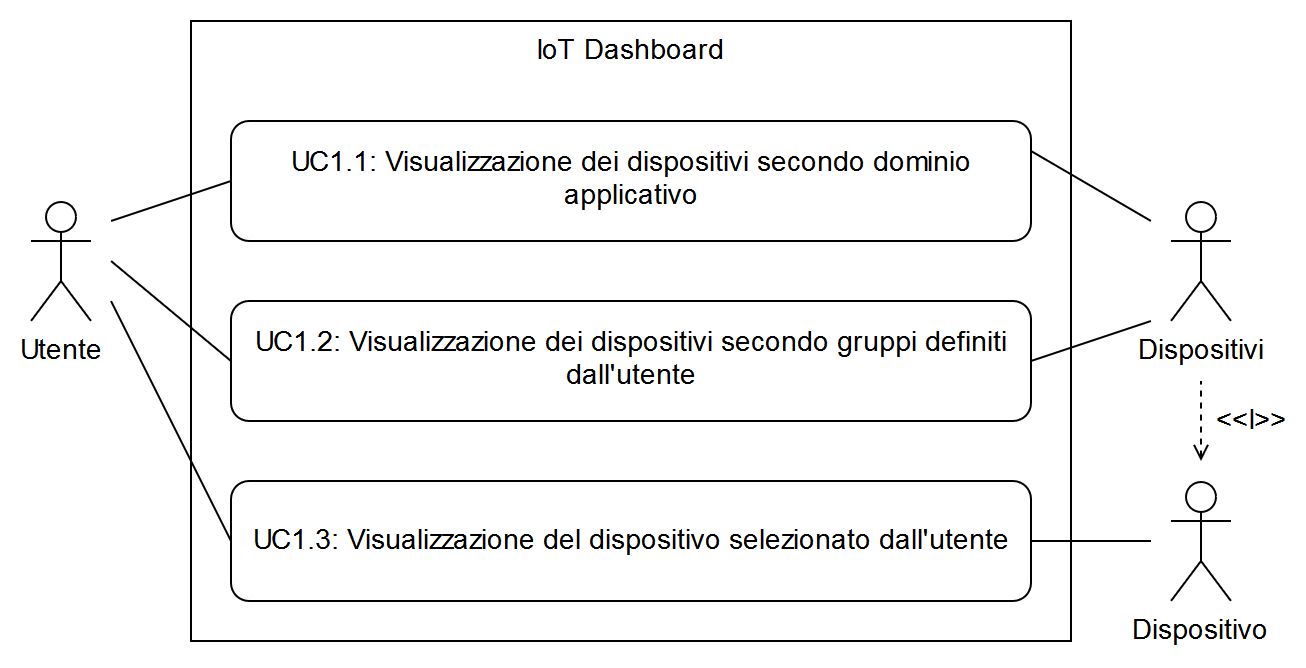
\includegraphics[width=0.9\columnwidth]{usecase/UC1}
    \caption{Use Case - UC1: Visualizzazione dei dispositivi collegati}
\end{figure}
% fine uc

% uc testuale
\begin{usecase}{1.1}{Visualizzazione dei dispositivi collegati secondo dominio applicativo}
\usecaseactors{Utente, Dispositivi}
\usecasepre{L'utente ha scelto di visualizzare tutti i dispositivi collegati}
\usecasedesc{L'utente interroga la \emph{dashboard} per conoscere lo stato dei dispositivi collegati. In questa visualizzazione la \emph{dashboard} mostra i dispositivi raggruppati secondo dominio applicativo (gruppo relativo alla termodinamica domestica, gruppo relativo alla illuminazione, ecc.)}
\usecasepost{L'utente conosce lo stato di tutti i dispositivi collegati al sistema secondo il dominio scelto}
\label{uc:uc1.1}
\end{usecase}
% fine uc

% uc testuale
\begin{usecase}{1.2}{Visualizzazione dei dispositivi collegati secondo gruppi definiti dall'utente}
\usecaseactors{Utente, Dispositivi}
\usecasepre{L'utente ha scelto di visualizzare tutti i dispositivi collegati}
\usecasedesc{L'utente interroga la \emph{dashboard} per conoscere lo stato dei dispositivi collegati. In questa visualizzazione la \emph{dashboard} mostra i dispositivi raggruppati secondo le preferenze dell'utente}
\usecasepost{L'utente conosce lo stato di tutti i dispositivi collegati al sistema presenti nel gruppo definito}
\label{uc:uc1.2}
\end{usecase}
% fine uc

% uc testuale
\begin{usecase}{1.3}{Visualizzazione del dispositivo selezionato dall'utente}
\usecaseactors{Utente, Dispositivi}
\usecasepre{L'utente ha scelto di visualizzare le informazioni di uno dei dispositivi collegati}
\usecasedesc{L'utente interroga la \emph{dashboard} per conoscere lo stato del dispositivo selezionato. In questa visualizzazione la \emph{dashboard} mostra le informazioni provenienti dal dispositivo}
\usecasepost{L'utente può visualizzare le informazioni specifiche del dispositivo}
\label{uc:uc1.3}
\end{usecase}
% fine uc

% uc testuale
\begin{usecase}{1.3.1}{Visualizzazione delle informazioni provenienti dal dispositivo}
\usecaseactors{Utente, Dispositivi}
\usecasepre{L'utente ha scelto di visualizzare le informazioni di uno dei dispositivi collegati}
\usecasedesc{La \emph{dashboard} mostra all'utente le informazioni provenienti dal dispositivo}
\usecasepost{L'utente può visualizzare le informazioni specifiche del dispositivo}
\label{uc:uc1.3.1}
\end{usecase}
% fine uc

% uc testuale
\begin{usecase}{1.3.1.1}{Visualizzazione nome del dispositivo}
\usecaseactors{Utente, Dispositivi}
\usecasepre{L'utente ha scelto di visualizzare le informazioni di uno dei dispositivi collegati}
\usecasedesc{La \emph{dashboard} mostra all'utente il nome \emph{user-friendly} dato dal produttore al dispositivo}
\usecasepost{L'utente conosce il nome dato dal produttore al dispositivo}
\label{uc:uc1.3.1.1}
\end{usecase}
% fine uc

% uc testuale
\begin{usecase}{1.3.1.2}{Visualizzazione categoria del dispositivo}
\usecaseactors{Utente, Dispositivi}
\usecasepre{L'utente ha scelto di visualizzare le informazioni di uno dei dispositivi collegati}
\usecasedesc{La \emph{dashboard} mostra all'utente il dominio applicativo del dispositivo (illuminazione, ecc.)}
\usecasepost{L'utente conosce il dominio applicativo del dispositivo selezionato}
\label{uc:uc1.3.1.2}
\end{usecase}
% fine uc

% uc testuale
\begin{usecase}{1.3.1.3}{Visualizzazione dati provenienti dal dispositivo}
\usecaseactors{Utente, Dispositivi}
\usecasepre{L'utente ha scelto di visualizzare le informazioni di uno dei dispositivi collegati}
\usecasedesc{La \emph{dashboard} mostra all'utente i dati raccolti dal sistema inviati dal dispositivo selezionato}
\usecasepost{L'utente conosce le misurazioni raccolte dal sistema per il dispositivo selezionato}
\label{uc:uc1.3.1.3}
\end{usecase}
% fine uc

% uc testuale
\begin{usecase}{1.3.2}{Visualizzazione delle specifiche tecniche del dispositivo}
\usecaseactors{Utente, Dispositivi}
\usecasepre{L'utente ha scelto di visualizzare le informazioni di uno dei dispositivi collegati}
\usecasedesc{La \emph{dashboard} mostra all'utente le specifiche tecniche del dispositivo, quali produttore, modello, ecc.}
\usecasepost{L'utente conosce le specifiche tecniche del dispositivo selezionato}
\label{uc:uc1.3.2}
\end{usecase}
% fine uc

% uc testuale
\begin{usecase}{1.3.2.1}{Visualizzazione produttore del dispositivo}
\usecaseactors{Utente, Dispositivi}
\usecasepre{L'utente ha scelto di visualizzare le specifiche tecniche di uno dei dispositivi collegati}
\usecasedesc{La \emph{dashboard} mostra all'utente il nome del produttore del dispositvo}
\usecasepost{L'utente conosce il nome del produttore del dispositivo selezionato}
\label{uc:uc1.3.2.1}
\end{usecase}
% fine uc

% uc testuale
\begin{usecase}{1.3.2.2}{Visualizzazione modello del dispositivo}
\usecaseactors{Utente, Dispositivi}
\usecasepre{L'utente ha scelto di visualizzare le specifiche tecniche di uno dei dispositivi collegati}
\usecasedesc{La \emph{dashboard} mostra all'utente il nome commerciale scelto dal produttore per il dispositivo}
\usecasepost{L'utente conosce il nome commerciale del dispositivo selezionato}
\label{uc:uc1.3.2.2}
\end{usecase}
% fine uc

% uc testuale
\begin{usecase}{1.3.2.3}{Visualizzazione revisione del dispositivo}
\usecaseactors{Utente, Dispositivi}
\usecasepre{L'utente ha scelto di visualizzare le specifiche tecniche di uno dei dispositivi collegati}
\usecasedesc{La \emph{dashboard} mostra all'utente un identificativo di versione del dispositivo (anno o  numero di versione)}
\usecasepost{L'utente conosce la revisione del dispositivo selezionato}
\label{uc:uc1.3.2.3}
\end{usecase}
% fine uc

% uc testuale
\begin{usecase}{1.3.3}{Visualizzazione delle operazioni disponibili per il dispositivo}
\usecaseactors{Utente, Dispositivi}
\usecasepre{L'utente ha scelto di visualizzare informazioni di uno dei dispositivi collegati}
\usecasedesc{La \emph{dashboard} mostra all'utente le funzionalità offerte dal dispositivo}
\usecasepost{L'utente conosce la lista delle funzionalità offerte dal dispositivo selezionato}
\label{uc:uc1.3.3}
\end{usecase}
% fine uc

% uc testuale
\begin{usecase}{1.3.4}{Collegamento all'interfaccia proprietaria del dispositivo}
\usecaseactors{Utente, Dispositivi, Interfaccia proprietaria}
\usecasepre{L'utente ha scelto di visualizzare le informazioni di uno dei dispositivi collegati}
\usecasedesc{La \emph{dashboard} mostra all'utente il collegamento all'interfaccia proprietaria del dispositivo}
\usecasepost{L'utentepuò seguire il collegamento per visualizzare l'interfaccia proprietaria del dispositivo selezionato}
\label{uc:uc1.3.4}
\end{usecase}
% fine uc

% uc testuale
\begin{usecase}{2}{Gestione dei dispositivi collegati}
\usecaseactors{Utente, Dispositivi}
\usecasepre{L'utente ha scelto di gestire i dispositivi collegati al sistema}
\usecasedesc{L'utente accede alla \emph{dashboard} per gestire i dispositivi collegati al sistema}
\usecasepost{L'utente può accedere alle funzionalità di gestione offerte dalla \emph{dashboard}}
\label{uc:uc2}
\end{usecase}

\begin{figure}[!h]
    \centering
    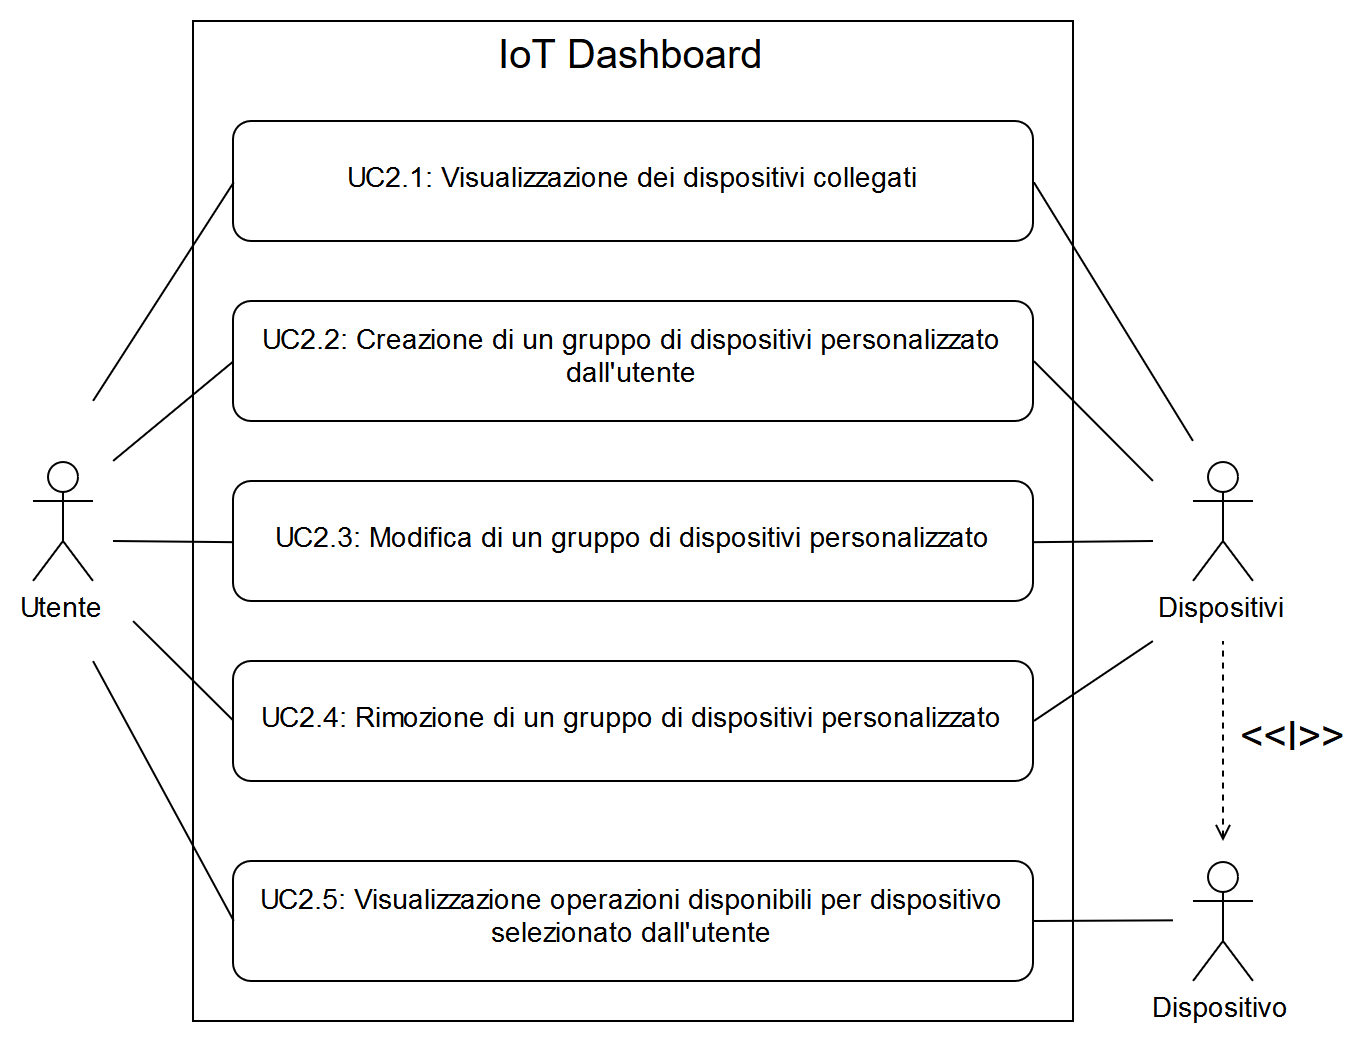
\includegraphics[width=0.9\columnwidth]{usecase/UC2}
    \caption{Use Case - UC2: Gestione dei dispositivi collegati}
\end{figure}
% fine uc

% uc testuale
\begin{usecase}{2.1}{Visualizzazione dei dispositivi collegati}
\usecaseactors{Utente, Dispositivi}
\usecasepre{L'utente ha scelto di gestire i dispositivi collegati al sistema}
\usecasedesc{La \emph{dashboard} presenta all'utente la lista di dispositivi collegati al sistema per permettere all'utente di selezionare quale dispositivo gestire}
\usecasepost{L'utente può accedere alle funzionalità di gestione offerte dalla \emph{dashboard} per i dispositivi visualizzati}
\label{uc:uc2.1}
\end{usecase}
% fine uc

% uc testuale
\begin{usecase}{2.2}{Creazione di un gruppo di dispositivi personalizzato dall'utente}
\usecaseactors{Utente, Dispositivi}
\usecasepre{L'utente ha scelto di gestire i dispositivi collegati al sistema}
\usecasedesc{La \emph{dashboard} permette all'utente di creare un gruppo personalizzato di dispositivi, facilitando la visualizzazione dei dispositivi nella pagina principale della \emph{dashboard}}
\usecasepost{L'utente ha creato un gruppo personalizzato con le proprietà richieste (nome e dispositivi)}
\label{uc:uc2.2}
\end{usecase}
% fine uc

% uc testuale
\begin{usecase}{2.2.1}{Inserimento nome del gruppo}
\usecaseactors{Utente}
\usecasepre{L'utente ha scelto di creare un gruppo personalizzato}
\usecasedesc{L'utente fornisce al sistema il nome del gruppo da creare}
\usecasepost{L'utente può proseguire nella creazione del gruppo personalizzato}
\label{uc:uc2.2.1}
\end{usecase}
% fine uc

% uc testuale
\begin{usecase}{2.2.2}{Scelta dei dispositivi da inserire nel gruppo}
\usecaseactors{Utente, Dispositivi}
\usecasepre{L'utente ha scelto di creare un gruppo personalizzato}
\usecasedesc{L'utente può selezionare i dispositivi che vuole raggruppare}
\usecasepost{L'utente ha creato un gruppo personalizzato con le proprietà specificate (nome e dispositivi)}
\label{uc:uc2.2.2}
\end{usecase}
% fine uc

% uc testuale
\begin{usecase}{2.3}{Modifica di un gruppo di dispositivi personalizzato}
\usecaseactors{Utente, Dispositivi}
\usecasepre{L'utente ha scelto di gestire i dispositivi collegati al sistema}
\usecasedesc{La \emph{dashboard} permette all'utente di modificare un gruppo personalizzato esistente per rinominare il gruppo e aggiungere o togliere uno o più dispositivi da un gruppo}
\usecasepost{L'utente ha modificato il gruppo personalizzato esistente}
\label{uc:uc2.3}
\end{usecase}
% fine uc

% uc testuale
\begin{usecase}{2.3.1}{Modifica nome del gruppo}
\usecaseactors{Utente}
\usecasepre{L'utente ha scelto di modificare un gruppo personalizzato esistente}
\usecasedesc{La \emph{dashboard} mostra all'utente il nome corrente del gruppo, permettendone la modifica}
\usecasepost{L'utente ha modificato il nome del gruppo personalizzato esistente}
\label{uc:uc2.3.1}
\end{usecase}
% fine uc

% uc testuale
\begin{usecase}{2.3.2}{Aggiunta di nuovi dispositivi al gruppo}
\usecaseactors{Utente, Dispositivi}
\usecasepre{L'utente ha scelto di modificare un gruppo personalizzato esistente}
\usecasedesc{La \emph{dashboard} permette all'utente di scegliere quali dispositivi non presenti nel gruppo aggiungere}
\usecasepost{L'utente ha aggiunto i dispositivi selezionati al gruppo personalizzato esistente}
\label{uc:uc2.3.2}
\end{usecase}
% fine uc

% uc testuale
\begin{usecase}{2.3.3}{Rimozione di dispositivi esistenti dal gruppo}
\usecaseactors{Utente, Dispositivi}
\usecasepre{L'utente ha scelto di modificare un gruppo personalizzato esistente}
\usecasedesc{La \emph{dashboard} permette all'utente di scegliere quali dispositivi presenti nel gruppo da rimuovere}
\usecasepost{L'utente ha rimosso i dispositivi selezionati al gruppo personalizzato esistente}
\label{uc:uc2.3.3}
\end{usecase}
% fine uc

% uc testuale
\begin{usecase}{2.4}{Rimozione di un gruppo di dispositivi personalizzato}
\usecaseactors{Utente}
\usecasepre{L'utente ha scelto di modificare un gruppo personalizzato esistente}
\usecasedesc{La \emph{dashboard} permette all'utente di rimuovere un gruppo personalizzato esistente}
\usecasepost{L'utente ha rimosso il gruppo personalizzato esistente selezionato}
\label{uc:uc2.4}
\end{usecase}
% fine uc

% uc testuale
\begin{usecase}{2.5}{Visualizzazione delle operazioni disponibili per il dispositivo selezionato dall'utente}
\usecaseactors{Utente, Dispositivo}
\usecasepre{L'utente ha scelto di modificare un gruppo personalizzato esistente}
\usecasedesc{La \emph{dashboard} permette all'utente di conoscere la lista delle operazioni disponibili per il dispositivo selezionato (ad esempio: accensione e spegnimento per una sorgente di illuminazione)}
\usecasepost{L'utente conosce la lista delle operazioni disponibili per il dispositivo selezionato}
\label{uc:uc2.5}
\end{usecase}
% fine uc

% uc testuale
\begin{usecase}{3}{Visualizzazione delle statistiche di sistema}
\usecaseactors{Utente}
\usecasepre{L'utente ha scelto di visualizzare lo stato del sistema}
\usecasedesc{L'utente interroga la \emph{dashboard} per visualizzare le statistiche di sistema per conoscerne lo stato di salute e diagnosticare eventuali malfunzionamenti}
\usecasepost{L'utente conosce lo stato del sistema}
\label{uc:uc3}
\end{usecase}
% fine uc

% ## Requisiti
Presento di seguito i requisiti emersi durante l’analisi dei casi d’uso.
Per permetterne una consultazione agevole, ho deciso di inserire i requisiti in una tabella dei requisiti ~\ref{tab:requisiti}.
Nella tabella ~\ref{tab:requisiti}, presento i requisiti indicando:
\begin{itemize}
	\item Identificativo (secondo le regole indicate successivamente);
	\item Categoria di appartenenza fra:
	\begin{itemize}
		\item Obbligatorio, per i requisiti irrinunciabili;
		\item Desiderabile, per i requisiti non strettamente necessari ma che offrono un
    valore aggiunto riconoscibile;
		\item Opzionale, per i requisiti relativamente utili o contrattabili in seguito.
	\end{itemize}
	\item Descrizione esaustiva del requisito;
\end{itemize}

\newenvironment{conditions}
  {\par\vspace{\abovedisplayskip}\noindent\begin{tabular}{>{$}l<{$} @{${}={}$} l}}
  {\end{tabular}\par\vspace{\belowdisplayskip}}

% ### Catalogazione requisiti
I requisiti sono identificati come segue:

\begin{figure}
  \centering
  \[ R[Categoria][Tipo][numero] \]
	dove
	\begin{conditions}
    R & specifica che si tratta di un requisito\\
    Categoria & indica se si tratta di un requisito tra quelli definiti in tabella ~\ref{tab:categoria-requisiti}\\
    Tipo & indica la tipologia del requisito tra quelli definiti in tabella ~\ref{tab:tipi-requisiti}\\
		Numero & è assoluto e rappresenta un riferimento univoco al requisito in questione\\
	\end{conditions}
\end{figure}

\begin{table}[H]
\caption{Tabella recante le categorie di requisiti}
\label{tab:categoria-requisiti}
\begin{tabularx}{\linewidth}{|c|X|}
\hline
\textbf{Identificativo} & \textbf{Descrizione e origine} \\
\hline
M & Obbligatorio (\emph{mandatory}) \\
\hline
A & Desiderabile ((\emph{advisable}) \\
\hline
O & Opzionale (\emph{optional}) \\
\hline
\end{tabularx}
\end{table}

\begin{table}[H]
\caption{Tabella recante i tipi di requisiti}
\label{tab:tipi-requisiti}
\begin{tabularx}{\linewidth}{|c|X|}
\hline
\textbf{Identificativo} & \textbf{Descrizione e origine} \\
\hline
O & Di vincolo (\emph{obligation}) \\
\hline
F & Funzionale (\emph{functional}) \\
\hline
Q & Di qualità (\emph{quality}) \\
\hline
\end{tabularx}
\end{table}

% ### Tabella dei requisiti

% #### Tabella dei requisiti di vincolo

\begin{table}[H]
\caption{Tabella dei requisiti di vincolo}
\label{tab:requisiti-vincolo}
\begin{tabularx}{\linewidth}{|c|c|X|}
\hline
\textbf{Identificativo} & \textbf{Categoria} & \textbf{Descrizione} \\
\hline
RMO1 & Obbligatorio & Il sistema deve essere progettato secondo lo stile di progettazione a microservizi. \\
\hline
RAO2 & Desiderabile & Il sistema può essere implementato utilizzando il linguaggio JavaScript secondo lo standard ECMAScript 2017. \\
\hline
RAO3 & Desiderabile & Il sistema può essere implementato utilizzando il \emph{framework} Node.js per il \emph{backend} e React per il \emph{frontend}. \\
\hline
RMO4 & Obbligatorio & Il sistema deve utilizzare il protocollo MQTT. \\
\hline
\end{tabularx}
\end{table}

% #### Tabella dei requisiti funzionali

\begin{table}[H]
\caption{Tabella dei requisiti funzionali}
\label{tab:requisiti-funzionali}
\begin{tabularx}{\linewidth}{|c|c|X|}
\hline
\textbf{Identificativo} & \textbf{Categoria} & \textbf{Descrizione} \\
\hline
RMF1 & Obbligatorio & L'utente deve poter visualizzare tutti i dispositivi collegati al sistema. \\
\hline
RMF2 & Obbligatorio & L'utente deve poter visualizzare i dispositivi collegati secondo dominio applicativo. \\
\hline
RAF3 & Desiderabile & L'utente può visualizzare i dispositivi collegati secondo gruppi personalizzati. \\
\hline
RMF4 & Obbligatorio & L'utente deve poter selezionare uno dei dispositivi collegati per visualizzarne le informazioni. \\
\hline
RAF5 & Desiderabile & L'utente può creare un gruppo di dispositivi personalizzato. \\
\hline
RAF6 & Desiderabile & L'utente può modificare uno dei gruppi personalizzati esistenti. \\
\hline
RAF7 & Desiderabile & L'utente può rimuovere uno dei gruppi di dispositivi personalizzati esistenti. \\
\hline
RMF8 & Obbligatorio & L'utente deve poter visualizzare le operazioni messe a disposizione dal dispositivo selezionato. \\
\hline
RMF9 & Obbligatorio & L'utente deve poter selezionare una delle operazioni disponibili. \\
\hline
RMF10 & Obbligatorio & L'utente deve poter visualizzare le statistiche di utilizzo del sistema sistema. \\
\hline
\end{tabularx}
\end{table}

% #### Tabella dei requisiti di qualità

\begin{table}[H]
\caption{Tabella dei requisiti di qualità}
\label{tab:requisiti-qualita}
\begin{tabularx}{\linewidth}{|c|c|>{\setlength\hsize{\hsize}}X|}
\hline
\textbf{Identificativo} & \textbf{Categoria} & \textbf{Descrizione} \\
\hline
ROQ1 & Opzionale & Il sistema deve essere testato, raggiungendo i seguenti obiettivi:
\begin{itemize}
	\item \emph{statement coverage} > 80 \%
	\item \emph{branch coverage} > 90 \%
\end{itemize}\\
\hline
\end{tabularx}
\end{table}

\begin{table}[H]
\caption{Tabella di riepilogo dei requisiti}
\label{tab:requisiti-riepilogo}
\begin{tabularx}{\linewidth}{|X|c|c|c|}
\hline
\textbf{Tipo} & \textbf{Obbligatorio} & \textbf{Opzionale} & \textbf{Desiderabile} \\
\hline
Funzionale & 6 & 0 & 4 \\
\hline
Qualitativo & 0 & 1 & 0 \\
\hline
Di vincolo & 2 & 0 & 2 \\
\hline
Totale & 8 & 1 & 6 \\
\hline
\end{tabularx}
\end{table}

\pagebreak

%**************************************************************
\section{Progettazione}

% ### Scopo del documento

In questa sezione del documento definisco la progettazione dell'architettura ad alto livello del progetto di stage.
La sezione include la descrizione dell'architettura del sistema e delle relative componenti \emph{software} e i Design Pattern utilizzati per la progettazione.

% ## Architettura

L'architettura scelta per il sistema segue lo stile architetturale a microservizi con l'obiettivo di approfondire questo stile architetturale e implementarlo in uno scenario plausibile.
Lo stile architetturale a microservizi descrive un metodo di progettazione delle applicazioni come insiemi di servizi eseguibili indipendentemente, che comunicano tra loro grazie a meccanismi di comunicazione leggeri.

Nell'immagine ~\ref{img:overview-arch} illustro la panoramica delle componenti di cui è composta l'architettura.

\begin{figure}[H]
    \centering
    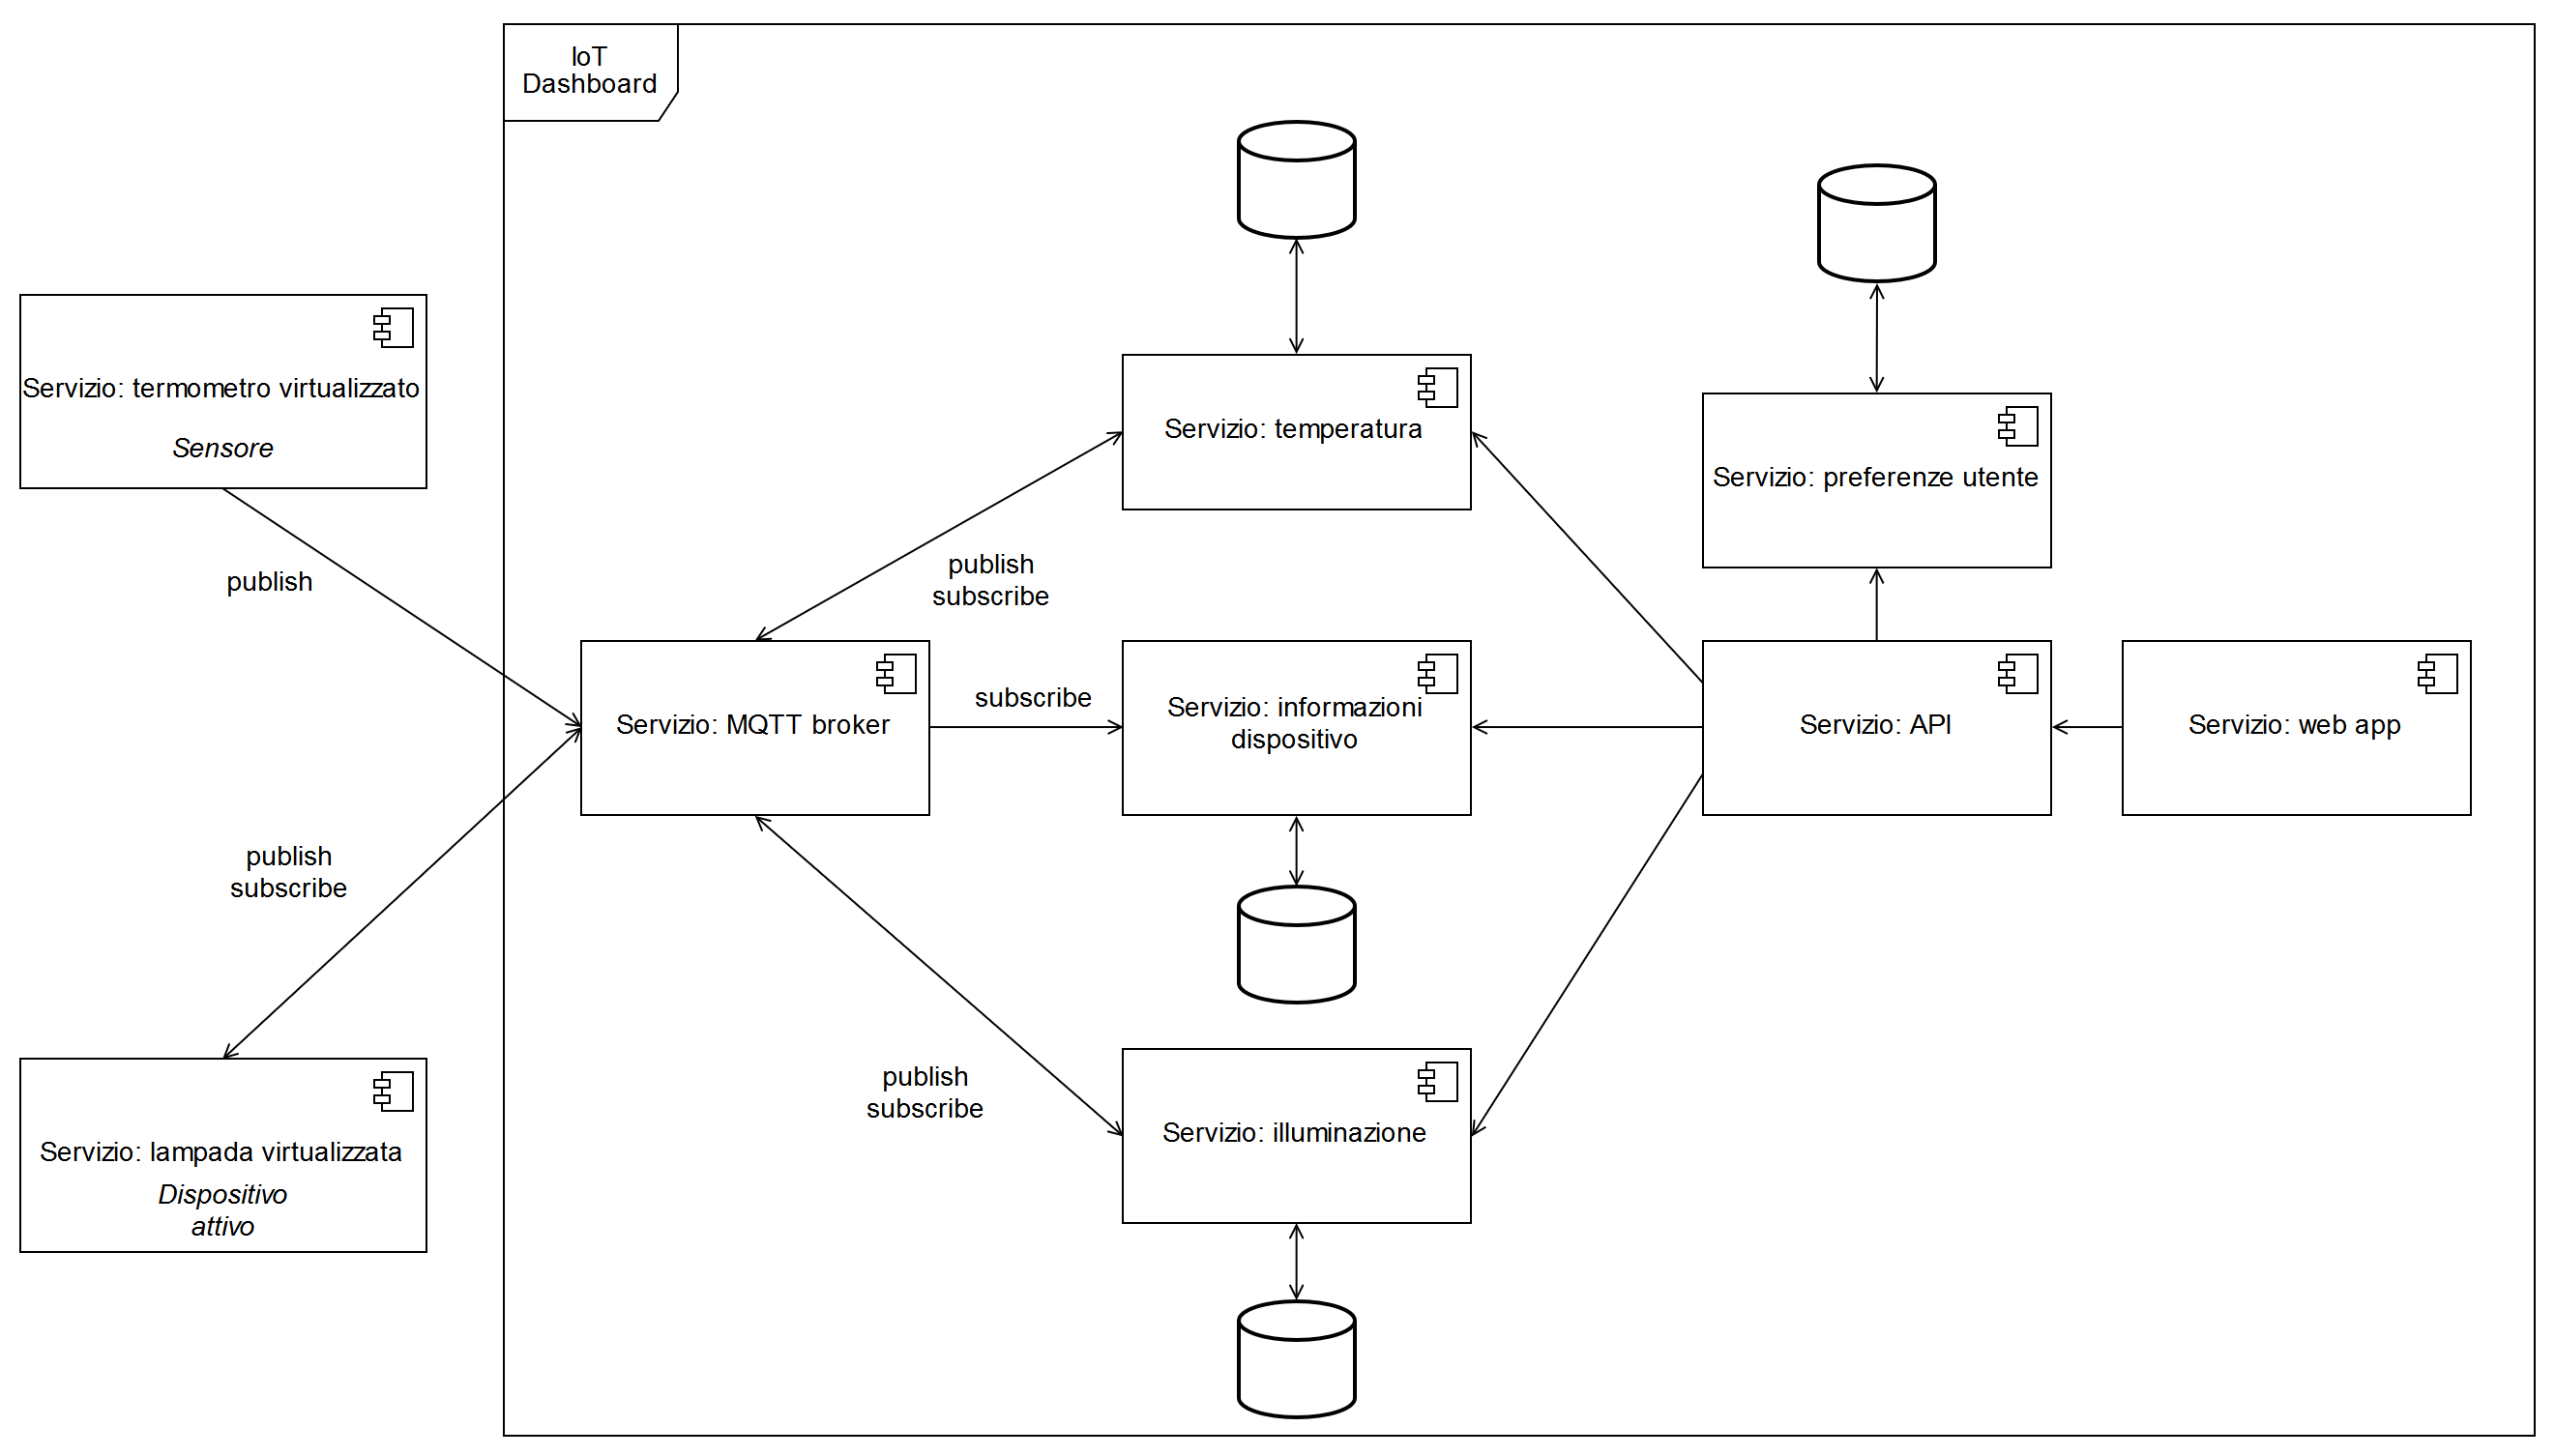
\includegraphics[width=\columnwidth]{progettazione/arch-overview}
    \caption{Panoramica dell'architettura ad alto livello progettata per il prototipo}
    \label{img:overview-arch}
\end{figure}

% ### Servizio: MQTT \emph{broker}

Il \emph{broker} MQTT è il servizio responsabile alla ricezione di tutti i messaggi, alla loro catalogazione e all'invio delle notifiche verso i \emph{client} sottoscritti a ciascuna categoria.
Il \emph{broker} memorizza lo stato di tutti i \emph{client} a lui connessi, inclusi i messaggi non ancora inviati o il cui invio è fallito.

% ### Servizio: termometro _virtualizzato_

Il termometro "virtualizzato" è il servizio responsabile alla simulazione di un sensore che invii dati sulla temperatura dell'ambiente in cui si trova.
Esso pubblica periodicamente la temperatura rilevata secondo l'argomento \emph{temperature}, mentre invia secondo l'argomento \emph{hw\_info} i propri dati identificativi, quali produttore, modello, ecc..
Data la relativa importanza i dati vengono inviati con un QoS di livello 0 nella categoria \emph{temperature}, mentre con QoS di livello 1 nella categoria \emph{hw\_info}.
In questo modo al collegamento del dispositvo "virtualizzato" viene effettuato almeno un tentativo di trasmissione delle informazioni relative alle specifiche del dispositivo.
Anche se nel diagramma è disegnato individualmente, è possibile che ve ne siano molteplici.
% #### Servizio: termometro _virtualizzato_ - Panoramica delle classi

Nella tabella ~\ref{tab:classi-termometro} sono elencate le classi sviluppate per soddisfare i requisiti di funzionamento del dispositivo.

\begin{table}[H]
\caption{Panoramica delle classi del servizio di simulazione del termometro "virtualizzato"}
\label{tab:classi-termometro}
\begin{tabularx}{\linewidth}{|c|X|}
\hline
\textbf{Classe} & \textbf{Funzionalità} \\
\hline
DeviceInfo & Classe i cui oggetti rappresentano le informazioni del dispositivo, quali produttore, modello, revisione, ecc. Questi dati vengono pubblicati nel \emph{topic} \emph{hw\_info}. \\
\hline
ServiceManager & Classe responsabile dell'integrazione tra generazione dei dati di temperatura, gestione delle informazioni del dispositivo e invio delle informazioni tramite protocollo MQTT. \\
\hline
MQTTClient & Classe utile all'inizializzazione del \emph{client} MQTT. \\
\hline
TemperatureCurveFactory & Classe Factory astratta che espone la funzionalità di creazione della curva di temperatura, rappresentata dalla classe `TemperatureCurve`. \\
\hline
SineTemperatureCurveFactory & Implementazione della factory `TemperatureCurveFactory` per la creazione di oggetti `SineTemperatureCurve`. \\
\hline
TemperatureCurve & Classe astratta che espone le funzionalità di inizializzazione della funzione, di aggiunta di rumore pseudocasuale nella funzione creata e di simulazione della temperatura data l'ora corrente. \\
\hline
SineTemperatureCurve & Classe che implementa `TemperatureCurve` definendo una funzione di simulazione sinusoidale, in cui i parametri modificabili sono ampiezza, frequenza e fase. \\
\hline
\end{tabularx}
\end{table}

% ### Servizio: temperatura

Il servizio relativo alla temperatura si occupa di raccogliere tutti i dati provenienti dai sensori di temperatura, memorizzandoli e mettendoli a disposizione in un formato strutturato per gli altri servizi del sistema.
Il servizio si sottoscrive alla categoria \emph{temperature} e comunica con un QoS di livello 0, inoltre può pubblicare messaggi con la sottocategoria \emph{temperature/active} per usufruire delle funzionalità aggiuntive presenti in dispositivi attivi legati alla temperatura, con un QoS di livello 1.
Nella tabella ~\ref{tab:classi-temperatura} sono elencate le classi sviluppate per soddisfare i requisiti di funzionamento del servizio di gestione dei dati collegati alla temperatura.

% #### Servizio: temperatura - Panoramica delle classi

\begin{table}[!h]
\caption{Panoramica delle classi del servizio relativo alla temperatura}
\label{tab:classi-temperatura}
\begin{tabularx}{\linewidth}{|c|X|}
\hline
\textbf{Classe} & \textbf{Funzionalità} \\
\hline
ServiceManager & Classe responsabile dell'integrazione tra ricezione dei dati di temperatura, gestione della persistenza dei dati ed esposizione di una interfaccia per gli altri servizi. \\
\hline
MQTTClient & Classe utile all'inizializzazione del \emph{client} MQTT. \\
\hline
DBClient & Classe utile all'inizializzazione del \emph{client} per il \emph{database} del servizio. \\
\hline
API & Classe che raccoglie le funzionalità esposte dal servizio. Le funzionalità esposte sono rappresentate in una lista di oggetti che rappresentano l'accesso alle risorse e le funzioni di reperimento ed elaborazione delle informazioni. \\
\hline
TemperatureData & Classe che rappresenta i dati ricevuti dai dispositivi attraverso il protocollo MQTT. Al suo interno sono definiti l'unità di misura utilizzata dal sensore e la temperatura ottenuta della misurazione del sensore. \\
\hline
\end{tabularx}
\end{table}

% ### Servizio: lampada _virtualizzata_

La lampada "virtualizzata" simula la presenza nella rete di un dispositivo "attivo": una lampada in grado di comunicare il proprio assorbimento energetico e la sua durata stimata.
La lista delle operazioni disponibili è la seguente:
\begin{itemize}
	\item accensione della lampada (QoS di livello 2);
	\item spegnimento della lampada (QoS di livello 2);
	\item richiesta assorbimento energetico (QoS di livello 0);
	\item richiesta tempo di vita stimato della lampada (QoS di livello 0).
\end{itemize}

Le operazioni di accensione e spegnimento della lampada necessitano di una affidabilità più elevata delle altre operazioni per evitare l'invio di richieste di accensione e spegnimento multiple.
L'argomento a cui la lampada si sottoscrive è \emph{light/active}, in quanto capace di rispondere a richieste più complesse. Al primo collegamento il dispositivo invia i propri dati identificativi, pubblicandoli nella categoria \emph{hw\_info}.
Nella tabella ~\ref{tab:classi-lampada} sono elencate le classi sviluppate per soddisfare i requisiti di funzionamento di una lampada "virtualizzata".

% #### Servizio: lampada _virtualizzata_ - Panoramica delle classi

\begin{table}[!h]
\caption{Panoramica delle classi del servizio di simulazione della lampada "virtualizzata"}
\label{tab:classi-lampada}
\begin{tabularx}{\linewidth}{|c|X|}
\hline
\textbf{Classe} & \textbf{Funzionalità} \\
\hline
DeviceInfo & Classe i cui oggetti rappresentano le informazioni del dispositivo, quali produttore, modello, revisione, ecc. Questi dati vengono pubblicati nel \emph{topic} \emph{hw\_info}. \\
\hline
ServiceManager & Classe responsabile dell'integrazione tra stato della lampada e invio delle informazioni tramite protocollo MQTT. \\
\hline
MQTTClient & Classe utile all'inizializzazione del \emph{client} MQTT. \\
\hline
Lamp & Classe che utilizza il Design Pattern \emph{Singleton} per fornire lo stato della lampada (on/off). \\
\hline
\end{tabularx}
\end{table}

% ### Servizio: illuminazione

Il servizio relativo all'illuminazione si occupa di raccogliere e memorizzare tutti i dati pubblicati dai dispositivi nella categoria \emph{light} e permette il controllo dei dispositivi sottoscritti alla categoria \emph{light/active}.
Questo servizio utilizza trasmissioni con tutti i livelli di QoS definiti nel protocollo MQTT: la comunicazione delle operazioni che l'utente esegue vengono trasmessi con il livello di affidabilità maggiore (Qos livello 2) per avere la garanzia che i dati trasmessi siano arrivati ai dispositivi atomicamente, la trasmissione delle specifiche tecniche del dispositivo vengono inviate con un livello di affidabilità intermedio (QoS livello 1) mentre le misurazioni vengono inviate nel modo più efficiente possibile (QoS livello 0).
Nella tabella ~\ref{tab:classi-illuminazione} sono elencate le classi sviluppate per soddisfare i requisiti di funzionamento del servizio di gestione dei dispositivi di illuminazione.

\begin{table}[!h]
\caption{Panoramica delle classi del servizio relativo all'illuminazione}
\label{tab:classi-illuminazione}
\begin{tabularx}{\linewidth}{|c|X|}
\hline
\textbf{Classe} & \textbf{Funzionalità} \\
\hline
ServiceManager & Classe responsabile dell'integrazione tra ricezione dei dati dei dispositivi di illuminazione, gestione della persistenza dei dati ed esposizione di una interfaccia per gli altri servizi. \\
\hline
MQTTClient & Classe utile all'inizializzazione del \emph{client} MQTT. \\
\hline
DBClient & Classe utile all'inizializzazione del \emph{client} per il \emph{database} del servizio. \\
\hline
API & Classe che rappresenta le funzionalità esposte dal servizio. Include i metodi di interfaccia per il controllo dei dispositivi di illuminazione "attivi". \\
\hline
LightData & Classe che rappresenta i dati ricevuti dai dispositivi attraverso il protocollo MQTT. Tra questi ci sono lo stato (on/off), il consumo alla rilevazione, l'intensità della luce emesse dalla lampada e la sua temperatura colore. \\
\hline
RGBLightDataDecorator & Classe che aggiunge informazioni relative alla temperatura colore della luce emessa dal dispositivo. \\
\hline
LightController & Classe che permette di controllare i dispositivi collegati, preparando i pacchetti che la classe `API` può inviare ai dispositivi secondo l'interfaccia definita dal produttore. \\
\hline
\end{tabularx}
\end{table}

% ### Servizio: informazioni dispositivo
Il servizio relativo alle informazioni dei dispositivi si occupa di raccogliere e memorizzare tutti i dati pubblicati secondo l'argomento \emph{hw\_info}.
Il servizio utilizza esclusivamente un livello di QoS pari a 1 per aumentare l'affidabilità del sistema a fronte delle attività di identificazione dei dispositivi collegati.
La tabella ~\ref{tab:classi-info} elenca le classi sviluppate per soddisfare i requisiti del servizio di identificazione dei dispositivi.

\begin{table}[H]
\caption{Panoramica delle classi del servizio relativo alle specifiche tecniche dei dispositivi connessi}
\label{tab:classi-info}
\begin{tabularx}{\linewidth}{|c|X|}
\hline
\textbf{Classe} & \textbf{Funzionalità} \\
\hline
ServiceManager & Classe responsabile dell'integrazione tra ricezione dei dati dei dispositivi, gestione della persistenza dei dati ed esposizione di una interfaccia per gli altri servizi. \\
\hline
MQTTClient & Classe utile all'inizializzazione del \emph{client} MQTT. \\
\hline
DBClient & Classe utile all'inizializzazione del \emph{client} per il \emph{database} del servizio. \\
\hline
API & Classe che rappresenta le funzionalità esposte dal servizio, permettendo di richiedere i dati dei dispositivi e fornire la specifica dei dati inviati dai dispositivi. \\
\hline
DeviceInfo & Classe che rappresenta le informazioni di base ricevute dai dispositivi attraverso il protocollo MQTT. Include il nome del produttore, il modello, la revisione e le informazioni tecniche di un dispositivo, quali intervallo di funzionamento, frequenza di misurazione, ecc. \\
\hline
ActiveDeviceOperations & Classe che contiene la lista delle operazioni messe a disposizione dai dispositivi "attivi". Ciascuna operazione contenuta nella lista è un'istanza della classe ActiveDeviceOperationDescriptor. \\
\hline
ActiveDeviceOperationDescriptor & Classe che contiene il nome della funzionalità emessa dal dispositivo e i possibili parametri che la funzionalità potrebbe richiedere. \\
\hline
\end{tabularx}
\end{table}

% ### Servizio: preferenze utente

Il servizio di gestione delle preferenze utente si occupa di salvare informazioni quali ad esempio gruppi personalizzati, unità di misura preferite, ecc.
Il servizio non utilizza il protocollo MQTT in quanto non richiede la comunicazione con i dispositivi connessi alla rete, quindi viene utilizzato solamente dal servizio API.
La tabella ~\ref{tab:classi-user} elenca le classi sviluppate per soddisfare i requisiti della gestione delle preferenze utente.

\begin{table}[!h]
\caption{Panoramica delle classi del servizio di gestione delle preferenze utente}
\label{tab:classi-user}
\begin{tabularx}{\linewidth}{|c|X|}
\hline
\textbf{Classe} & \textbf{Funzionalità} \\
\hline
ServiceManager & Classe responsabile della gestione della persistenza delle preferenze utente e dell'esposizione di una interfaccia per gli altri servizi. \\
\hline
DBClient & Classe utile all'inizializzazione del \emph{client} per il \emph{database} del servizio. \\
\hline
API & Classe che rappresenta le funzionalità esposte dal servizio, permettendo di richiedere e modificare le preferenze dell'utente. Espone inoltre la funzionalità di conversione dell'unità di misura verso quella predefinita dall'utente. \\
\hline
UserData & Classe che rappresenta le informazioni di base dell'utente (nome, cognome, ecc.). \\
\hline
SystemUnitDefinition & Classe che contiene l'elenco delle unità di misura scelte dall'utente per ogni metrica. \\
\hline
UnitsConverter & Classe che espone la funzionalità di conversione tra unità di misura compatibili. \\
\hline
\end{tabularx}
\end{table}

% ### Servizio: API

Il servizio API svolge un ruolo da intermediario tra il servizio che fornisce l'applicazione \emph{web} e il \emph{broker} MQTT.
Esso interroga i servizi "illuminazione", "temperatura" e "informazioni dispositivo"  definiti dal sistema per fornire una interfaccia unificata ai dati, sia in maniera sincrona sia in maniera asincrona.
L'interfaccia sincrona consiste in un'interfaccia che risponde ai metodi HTTP, mentre l'interfaccia asincrona richiede l'istituzione di una connessione che utilizzi i WebSocket.
Il servizio API nella sua funzione è l'implementazione di uno dei Design Pattern specifici per le architetture a microservizi, ossia il \emph{Gateway Pattern}.
Ho progettato il servizio API in modo \emph{stateless} grazie alla composizione delle API esposte dagli altri servizi: le chiamate effettuate al servizio API vengono dirottate ai rispettivi servizi e opportunamente decorate con informazioni aggiuntive, utili durante le attività di \emph{debug} del prototipo.
La tabella ~\ref{tab:classi-api} elenca le classi sviluppate per fornire le funzionalità richieste dai \emph{client} della \emph{dashboard}.

\begin{table}[!h]
\caption{Panoramica delle classi del servizio API}
\label{tab:classi-api}
\begin{tabularx}{\linewidth}{|c|X|}
\hline
\textbf{Classe} & \textbf{Funzionalità} \\
\hline
ServiceManager & Classe responsabile dell'integrazione tra istanza del server e interfaccia ai dati esposta. \\
\hline
Server & Classe responsabile del ciclo di vita del server Node.js. Nella classe Server attribuisco la lista delle risorse accessibili dai \emph{client} definiti nelle varie istanze di Route. \\
\hline
API & Classe che rappresenta le funzionalità esposte dal servizio, permettendo di richiedere e modificare le preferenze dell'utente. Espone inoltre la funzionalità di conversione dell'unità di misura verso quella predefinita dall'utente. \\
\hline
Route & Interfaccia che espone i metodi e le proprietà necessarie alla creazione delle risorse di accesso ai dati definite secondo lo stile architetturale REST. \\
\hline
UserRoute & Implementazione di `Route` che espone le risorse per la gestione delle preferenze utente. \\
\hline
DevicesRoute & Implementazione di `Route` che espone le risorse per la ricerca e identificazione dei dispositivi collegati. \\
\hline
TemperatureRoute & Implementazione di `Route` che espone le funzionalità di gestione della temperatura. \\
\hline
LightRoute & Implementazione di `Route` che espone le funzionalità di gestione dell'illuminazione. \\
\hline
\end{tabularx}
\end{table}

% ### Servizio: web app

Il servizio "\emph{web app}" comprende l'applicazione \emph{web} per la consultazione della \emph{dashboard} attraverso la navigazione tramite \emph{browser}.
Richiede i dati direttamente al servizio API utilizzando le interfacce REST esposte.
Questo servizio include i componenti sviluppati in React per la costruzione dell'interfaccia grafica della \emph{dashboard} e le classi necessarie alla sua pubblicazione sul \emph{web}.
La tabella ~\ref{tab:classi-web} elenca le classi sviluppate per implementare la \emph{dashboard}.

\begin{table}[!h]
\caption{Panoramica delle classi del servizio API}
\label{tab:classi-web}
\begin{tabularx}{\linewidth}{|c|X|}
\hline
\textbf{Classe} & \textbf{Funzionalità} \\
\hline
ServiceManager & Classe responsabile dell'integrazione tra istanza del server, pagine esposte e interfaccia di richeista dati. \\
\hline
DataFetcher & Modulo che si occupa di effettuare le richieste al servizio **API** secondo le definizioni fornite dal servizio. \\
\hline
Server & Classe responsabile del ciclo di vita del server Node.js. Effettua le richieste definite dalle istanze di `UIRoute` per ricevere i dati, utilizzando un'istanza di `DataFetcher`. \\
\hline
UIRoute & Interfaccia utilizzata per definire le richieste da effettuare per ricevere le informazioni che popolano le pagine della rotta. \\
\hline
UserUIRoute & Implementazione di `UIRoute` che definisce le richieste per ottenere o modificare le preferenze dell'utente ed espone le pagine di visualizzazione e modifica delle preferenze utente. \\
\hline
DevicesUIRoute & Implementazione di `UIRoute` che definisce le richieste per ottenere informazioni sui dispositivi collegati ed espone le pagine di visualizzazione di questi. \\
\hline
TemperatureUIRoute & Implementazione di `UIRoute` che definisce le richieste per ottenere dati legati alla temperatura, visualizzare ed eseguire operazioni con dispositivi attivi e ne permette la visualizzazione. \\
\hline
LightUIRoute & Implementazione di `UIRoute` che definisce le richieste per ottenere dati legati all'illuminazione, visualizzare ed eseguire operazioni con dispositivi attivi e ne permette la visualizzazione. \\
\hline
UIPage & Implementazione di un componente React (`React.Component`) che rappresenta una pagina. La pagina visualizzata può contenere più figli anch'essi componenti React. \\
\hline
React.Component & Classe che rappresenta un componente grafico nel \emph{framework} React. \\
\hline
\end{tabularx}
\end{table}

\pagebreak

% ## Design Pattern
I Design Pattern descrivono la metodologia con cui affrontare problemi ricorrenti, fornendo soluzioni standard condivise.
La conoscenza dei Design Pattern favorisce la progettazione, il riuso e la manutenibilità del codice prodotto.
I principali Design Pattern vengono suddivisi in quattro categorie:
\begin{itemize}
	\item Architetturali: affrontano il problema di progettazione di un sistema \emph{software} fornendo uno schema di partenza su cui basare l’architettura;
	\item Creazionali: affrontano il problema di astrarre il sistema rendendolo indipendente dall’implementazione concreta delle sue componenti;
	\item Strutturali: affrontano il problema riguardante la composizione delle classi e degli oggetti, sfruttando l’ereditarietà e l’aggregazione;
	\item Comportamentali: affrontano il problema dell’interazione tra le componenti, definendo la funzione degli oggetti e il modo in cui interagiscono gli uni con gli altri.
\end{itemize}

Tra i Design Pattern comportamentali, il Design Pattern Mediator ha l'intento di disaccoppiare entità del sistema che devono comunicare fra loro. Il pattern infatti fa in modo che queste entità non si referenzino reciprocamente, agendo da "mediatore" fra le parti.
Ho impiegato il Design Pattern Mediator in tutti i servizi sottoforma della classe `ServiceManager` per aumentare il disaccoppiamento tra classi che trattano la persistenza, l'esecuzione dei servizi, la comunicazione, ecc.

Tra i Design Pattern creazionali, ho utilizzato i pattern Abstract Factory e Singleton.
Il Design Pattern Abstract Factory fornisce un'interfaccia per creare famiglie di oggetti connessi o dipendenti tra loro, in modo che non ci sia necessità da parte dei \emph{client} di specificare quale classe istanziare. Questo pattern permette che un sistema sia indipendente dall'implementazione degli oggetti concreti e che il \emph{client}, attraverso l'interfaccia, utilizzi diverse famiglie di prodotti.
Ho utilizzato il Design Pattern Abstract Factory nel servizio di simulazione di un termometro (riferimento ~\ref{tab:classi-termometro}) per permettere la creazione di funzioni per la generazione della temperatura.
Il Design Pattern Singleton ha lo scopo di garantire che di una determinata classe venga creata una e una sola istanza, fornendo un unico punto di accesso globale a tale istanza.
Ho utilizzato il Design Pattern Singleton nel servizio di simulazione della lampada (riferimento ~\ref{tab:classi-lampada}) per obbligare il servizio a simulare una singola lampada, favorendo così l'esecuzione di numerosi \emph{container} del servizio per simulare un intero sistema d'illuminazione.

Tra i Design Pattern strutturali, ho utilizzato i pattern Decorator e Composite.
Il Design Pattern Decorator consente di aggiungere nuove funzionalità ad oggetti già esistenti, senza utilizzare l'ereditarietà tra classi.
Ho utilizzato il Design Pattern Decorator nel servizio relativo all'illuminazione (riferimento ~\ref{tab:classi-illuminazione}) per permettere al servizio di aggiungere dinamicamente le funzionalità di indicazione della temperatura colore di una sorgente luminosa.
Il Design Pattern Composite organizza gli oggetti in una struttura ad albero, nella quale i nodi sono delle entità composte e le foglie sono oggetti semplici.
Ho utilizzato il Design Pattern Composite nel servizio responsabile alla visualizzazione dell'interfaccia grafica (riferimento ~\ref{tab:classi-web}) per permettere la composizione di più componenti React per costruire interfacce complesse.

Il Design Pattern Module è uno dei pattern specifici del linguaggio JavaScript che ho utilizzato in tutti i servizi: il suo scopo è quello di rendere disponibile all’interno degli oggetti JavaScript l’incapsulazione, mantenendo privati e non accessibili dall’esterno campi dati e funzioni utilizzate internamente.

%**************************************************************
\section{Documentazione}

I documenti prodotti durante lo svolgimento dello stage sono in ordine:
\begin{enumerate}
	\item documento in cui descrivo il Piano di Lavoro del progetto di stage;
	\item documenti riguardanti la formazione:
		\begin{enumerate}
			\item documento in cui elenco i princìpi delle archietture a microservizi;
			\item documento in cui elenco le caratteristiche principali di Node.js;
			\item documento in cui elenco le caratteristiche principali di React;
			\item documento in cui riprendo un esercizio esistente per l'implementazione di una semplice architettura a microservizi;
		\end{enumerate}
		\item documenti di analisi dei protocolli considerati:
		\begin{enumerate}
			\item documento in cui analizzo le caratteristiche principale di MQTT;
			\item documento in cui analizzo le caratteristiche principali di Aeron (\url{https://github.com/real-logic/aeron});
		\end{enumerate}
		\item documento di Analisi dei Requisiti del prototipo;
		\item documento di Specifica Tecnica del prototipo;
		\item documenti in cui indico le risorse esposte dai servizi;
		\item documenti in cui elenco le istruzioni per eseguire il progetto in una macchina locale.
\end{enumerate}
Come menzionato nella sotto-sezione ~\ref{subsec:atom}, ho redatto tutti i documenti menzionati utilizzando l'\emph{editor} Atom.
I documenti relativi alla formazione sono rivolti essenzialmente al docente che mi ha seguito durante lo svolgimento dello stage e ad eventuali utenti che volessero approfondire i contenuti teorici su cui ho basato il prototipo.
Per i documenti di analisi, di progettazione e relativi alle risorse esposta dai servizi ho deciso di destinarli agli utenti che volessero approfondire il funzionamento del prototipo da un punto di vista ad alto livello.
I documenti in cui indico le risorse esposte dai servizi sono rivolti agli utenti più esperti che vogliono approfondire le funzionalità offerte dai servizi. Nelle mie previsioni questi utenti grazie ai documenti di specifica dovrebbero essere in grado di implementare le altre componenti del sistema, sostituendo le componenti da me implementate.
Per i documenti in cui indico le istruzioni per eseguire il progetto ho deciso di scrivere tali istruzioni sia in lingua italiana, sia in lingua inglese dal momento che il progetto è disponibile pubblicamente su GitHub. Le istruzioni contengono inoltre i riferimenti per installare i \emph{software} richiesti e ho fatto in modo che i procedimenti da seguire fossero i più brevi possibili (procedimenti con al massimo 5 istruzioni da seguire).
Ho scritto la documentazione del codice sorgente contestualmente al codice sorgente; la documentazione del codice sorgente consiste in commenti nei sorgenti JavaScript in cui spiego:
\begin{itemize}
	\item lo scopo delle proprietà degli oggetti;
	\item il tipo delle proprietà degli oggetti: in questo caso ho preferito annotare il tipo delle proprietà degli oggetti nella documentazione in quanto JavaScript non è staticamente tipizzato e quindi la dichiarazione di variabili non consente di specificare un tipo con cui il compilatore e l'interprete validi il codice sorgente;
	\item gli algoritmi utilizzati per l'implementazione delle funzionalità.
\end{itemize}
I commenti nel codice sorgente, come da \emph{best practice} per i progetti distribuiti pubblicamente, sono scritti in lingua inglese.

\pagebreak

%**************************************************************
\section{Test}

Ho progettato i test per raggiungere la copertura del codice fissata durante l'attività di Analisi dei Requisiti (riferimento ~\ref{tab:requisiti-qualita}).
Durante la progettazione dei test ho scelto di approfondire la progettazione dei test d'unità di tutte le componenti progettate come primo \emph{step} mentre ho tralasciato la progettazione dei test d'integrazione dei servizi: ho perseguito questa scelta perché ho ritenuto più importante aumentare l'affidabilità intrinseca di ciascun servizio indipendentemente dagli altri.
Uno dei fattori che mi ha consentito di effetuare questa scelta consiste nell'individualità dell'implementazione del progetto: se al progetto avessero collaborato uno o più sviluppatori, avrebbe assunto maggiore importanza la corretta interazione tra i servizi. Inoltre, dal momento che i servizi che ho progettato hanno un flusso dei dati ben definito, mi ha permesso di tenere allineate le modifiche attraverso i servizi in efficienza.
Nei test ho usato ampiamente \emph{mock} e \emph{stub} per isolare le eventuali dipendenze tra un modulo e un altro all'interno dello stesso servizio. Come avevo previsto durante lo studio degli argomenti, la componente in cui ho avuto alcune difficoltà nell'implementazione dei test consiste nei moduli che dialogano con un \emph{database}: per arginare il problema ho utilizzato librerie accessorie presenti su npm per simulare le risposte che i \emph{database} inviano nel caso in cui si verifichino errori. In questo modo ho potuto testare con successo anche eventuali malfunzionamenti relativi al collegamento con i \emph{database}.
Ho elencato i risultati della copertura del codice raggiunta al termine dello stage nella tabella ~\ref{tab:coverage}.

\begin{table}[H]
\caption{Tabella che specifica la copertura del codice raggiunta per ciascun servizio}
\label{tab:coverage}
\begin{tabularx}{\linewidth}{|X|c|c|}
\hline
\textbf{Servizio} & \textbf{\emph{Statement coverage}} & \textbf{\emph{Branch coverage}} \\
\hline
MQTT Broker & 93 \% & 90 \% \\
\hline
Sensore di temperatura "virtualizzato" & 97 \% & 85 \% \\
\hline
Temperatura & 92 \% & 81 \% \\
\hline
Lampada \emph{smart} "virtualizzata" & 83 \% & 67 \% \\
\hline
Illuminazione & 91 \% & 65 \% \\
\hline
Informazioni dispositivi & 90 \% & 77 \% \\
\hline
Preferenze utente & 90 \% & 79 \% \\
\hline
API & 70 \% & 70 \% \\
\hline
Applicazione \emph{web} & 50 \% & 63 \% \\
\hline
\textbf{Totale} & 85,44 \% & 75,22 \% \\
\hline
\end{tabularx}
\end{table}

%**************************************************************
\section{Validazione dei Requisiti}

Nella tabella ~\ref{tab:validazione-requisiti}) ho elencato lo stato dell'implementazione dei requisiti citati in Analisi (riferimento ~\ref{ar})).

\begin{table}[H]
\caption{Tabella dei requisiti funzionali}
\label{tab:validazione-requisiti}
\begin{tabularx}{\linewidth}{|c|c|X|}
\hline
\textbf{Identificativo} & \textbf{Categoria} & \textbf{Implementazione} \\
\hline
RMF1 & Obbligatorio & Fatto \\
\hline
RMF2 & Obbligatorio & Fatto \\
\hline
RAF3 & Desiderabile & Rigettato \\
\hline
RMF4 & Obbligatorio & Fatto \\
\hline
RAF5 & Desiderabile & Rigettato. \\
\hline
RAF6 & Desiderabile & Rigettato. \\
\hline
RAF7 & Desiderabile & Rigettato \\
\hline
RMF8 & Obbligatorio & Fatto \\
\hline
RMF9 & Obbligatorio & Fatto \\
\hline
RMF10 & Obbligatorio & Parziale \\
\hline
ROQ1 & Opzionale & Fatto \\
\hline
RMO1 & Obbligatorio & Fatto \\
\hline
RAO2 & Desiderabile & Fatto \\
\hline
RAO3 & Desiderabile & Fatto \\
\hline
RMO4 & Obbligatorio & Fatto \\
\hline
\end{tabularx}
\end{table}

Durante lo svolgimento dello stage ho deciso di non implementare i requisiti relativi alla personalizzazione dei gruppi di dispositivi perché ho incontrato alcune difficoltà relative alla composizione dei servizi che hanno rallentato l'implementazione delle funzionalità dei servizi. Ho scelto di non implementare queste funzionalità perchè, sebbene le avessi catalogate come desiderabili, la quantità di risorse non sarebbe stata sufficiente alla loro corretta implementazione, quindi ho preferito allocare tempo per migliorare la qualità del \emph{software} sviluppato aumentando la copertura del codice sorgente, implementando un numero maggiore di test di unità.
Per il requisito RMF10, relativo alla visualizzazione delle statistiche di sistema, ho deciso di implementare solamente la componente di controllo della salute dei servizi che compongono il sistema \emph{healthcheck}, tralasciando le componenti di integrazione dei dati raccolti dai servizi e le componenti di visualizzazione dei dati citati.
